\section{FrontEnd Implementation}
\label{secD4:FrontEndImplementation}
Il FrontEnd, (visualizzabile e utilizzabile al link \href{https://plan-it.it} {https://plan-it.it}) implementato in questo prototipo del sito PlanIt da noi sviluppato, fornisce le funzionalità di visualizzazione, creazione, modifica e cancellazione di calendari ed eventi all'interno dell'applicativo; gli eventi che si possono gestire, in questo prototipo, sono solo singoli, ovvero che in fase di creazione o modifica vengono definiti solo per una specifica data.
\begin{comment}
, oppure eventi ripetuti, ovvero che vengono definiti per più giornate in fase di creazione o modifica. 
\end{comment}
Inoltre, dopo il primo accesso, è presente anche l'automatica creazione di un account per l'utente che ha fatto la registrazione e viene anche data la possibilità di modificare il proprio username, che nel caso non venisse definito, corrisponde alla propria email. \\ Prima di cominciare con la descrizione più specifica di ciascuna schermata, partiamo con il dire che le pagine che costituiscono questo prototipo del sito PlanIt, sono: "Homepage", "schermata login", "schermata registrazione", "schermata recupero password", "schermata inserimnento soprannome", "schermata Calendario" e "schermata Eventi".
\\ In particolare partiamo da come appare il sito, quando ci si accede. La prima pagina che si visualizza, è l'Homepage, visualizzabile nell'immagine sottostante. Dall' "Homepage", l'utente può solo premere il tasto "Login", che lo indirizzerà alla pagina di autenticazione fornita da Auth0. Infatti tutta la fase di registrazione, login e anche recupero password sono gestite completamente da questo sistema esterno di autenticazione che integriamo nel sito. Il bottone "Try Demo", presente nell' "Homepage", non ha nessuna funzionalità, in quanto in questo prototipo del sito, si è sviluppato solo il sito per gli utenti che si autenticano.
\begin{center}
    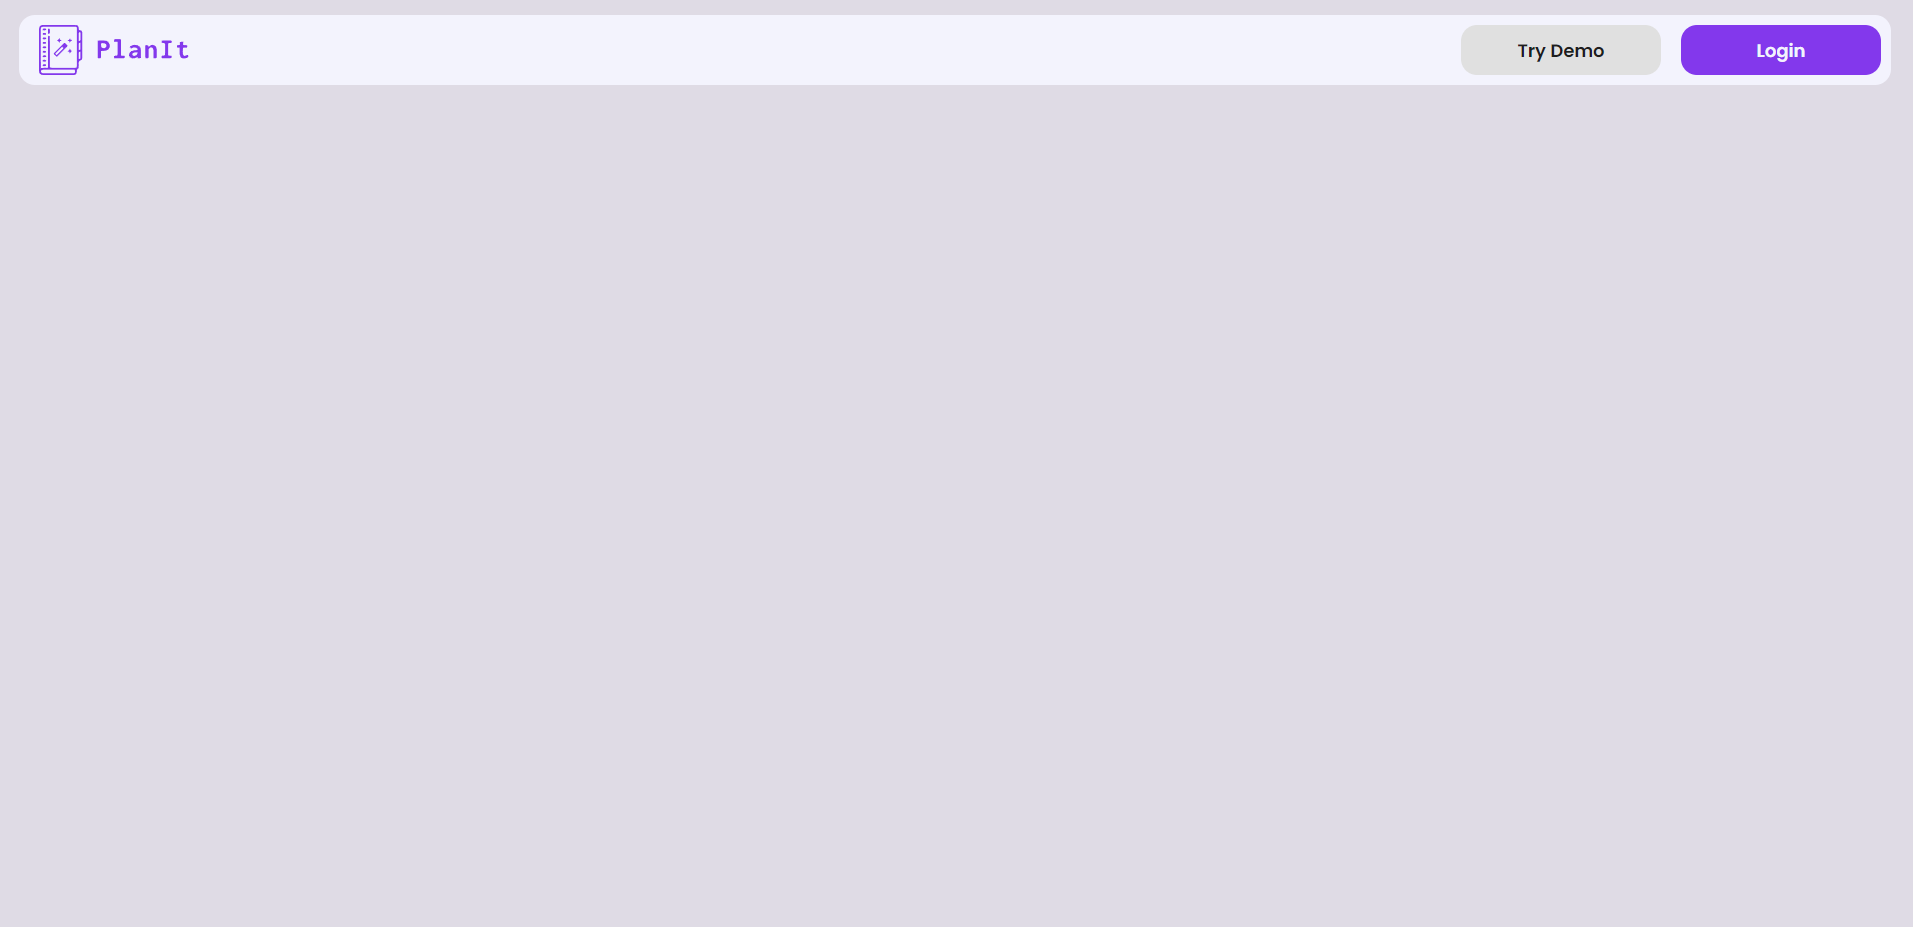
\includegraphics[width=1\textwidth, height=0.3\textheight]{img/png/FrontEnd/Homepage_Autenticazione/Homepage.png}
    \captionof{figure}{FrontEnd - Homepage}
    \blfootnote{Immagine \href{https://github.com/Life-planner/Documentazione/blob/main/D4/img/png/FrontEnd/Homepage_Autenticazione/Homepage.png}{PNG} FrontEnd - Homepage}
\end{center}
Quindi, dopo aver premuto il bottone "Login", si è indirizzati nella pagina dove avviene il login, che si può osservare qua sotto. In questa pagina, se l'utente ha già un proprio account PlanIt, può accedere usando le sue credenziali, oppure l'autenticazione può esser fatta usando anche un account Google appartenente all'utente che vuole accedere al sito PlanIt come utente autenticato. Ovviamente, nel caso si provasse a fare l'accesso mediante credenziali, ma si inserissero delle credenziali errate, il sistema notifica l'utente dell'errore che si è verificato.
\begin{center}
    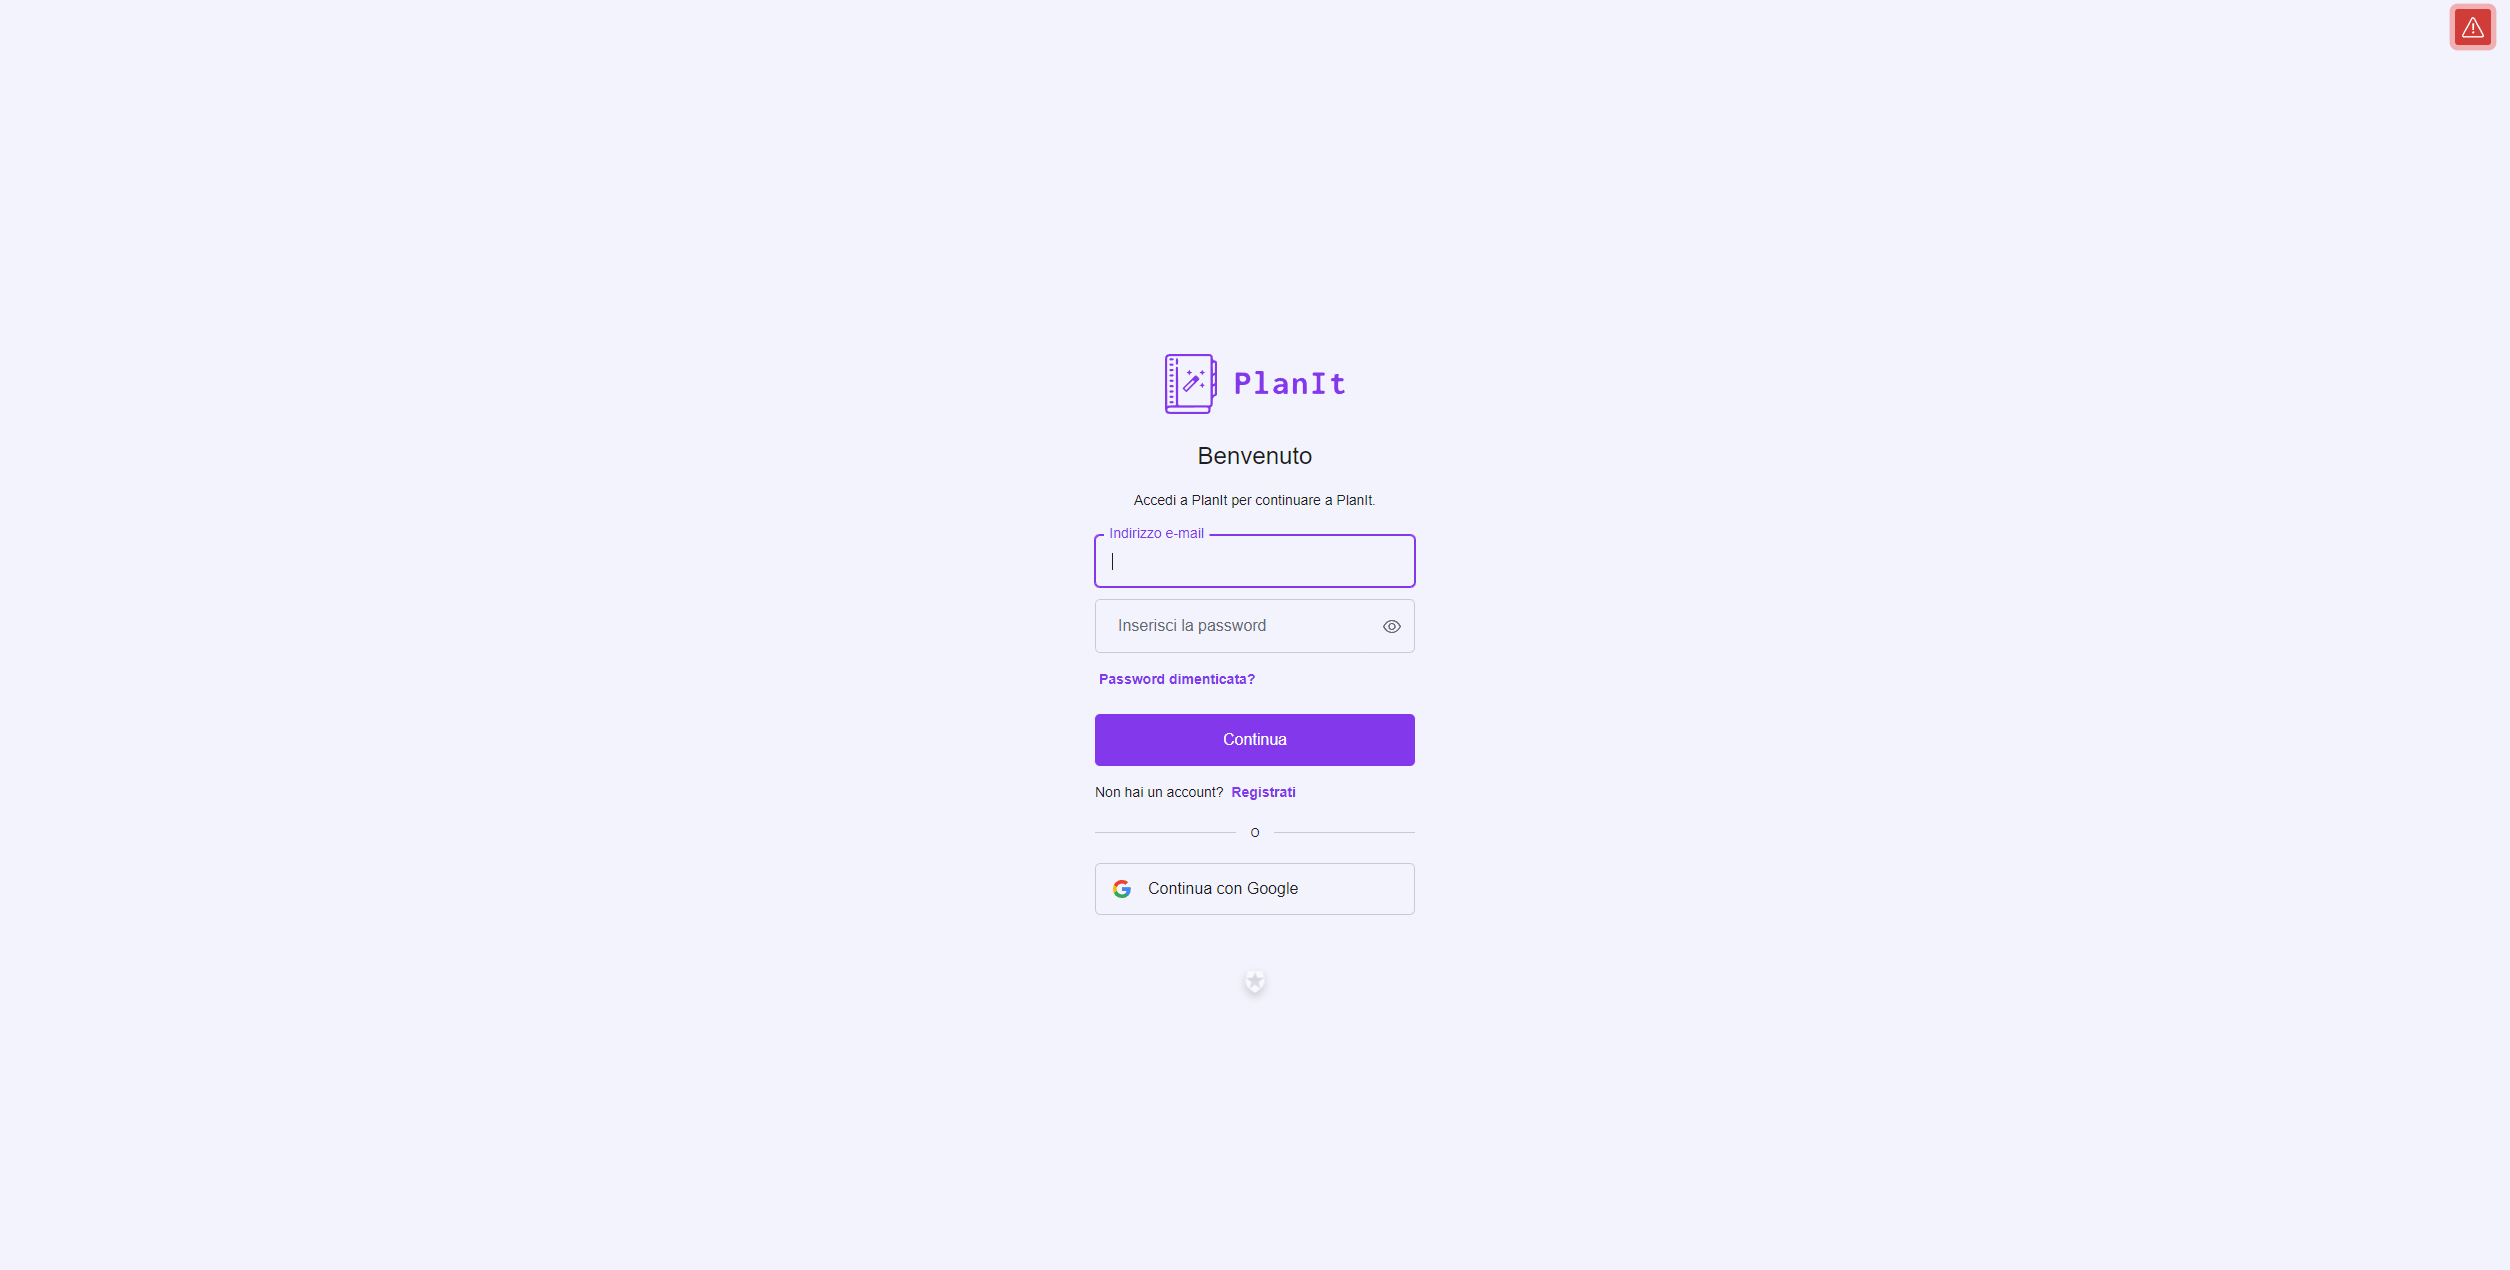
\includegraphics[width=1\textwidth, height=0.3\textheight]{img/png/FrontEnd/Homepage_Autenticazione/login.png}
    \captionof{figure}{FrontEnd - Login}
    \blfootnote{Immagine \href{https://github.com/Life-planner/Documentazione/blob/main/D4/img/png/FrontEnd/Homepage_Autenticazione/login.png}{PNG} FrontEnd - Login}
\end{center}

\begin{center}
    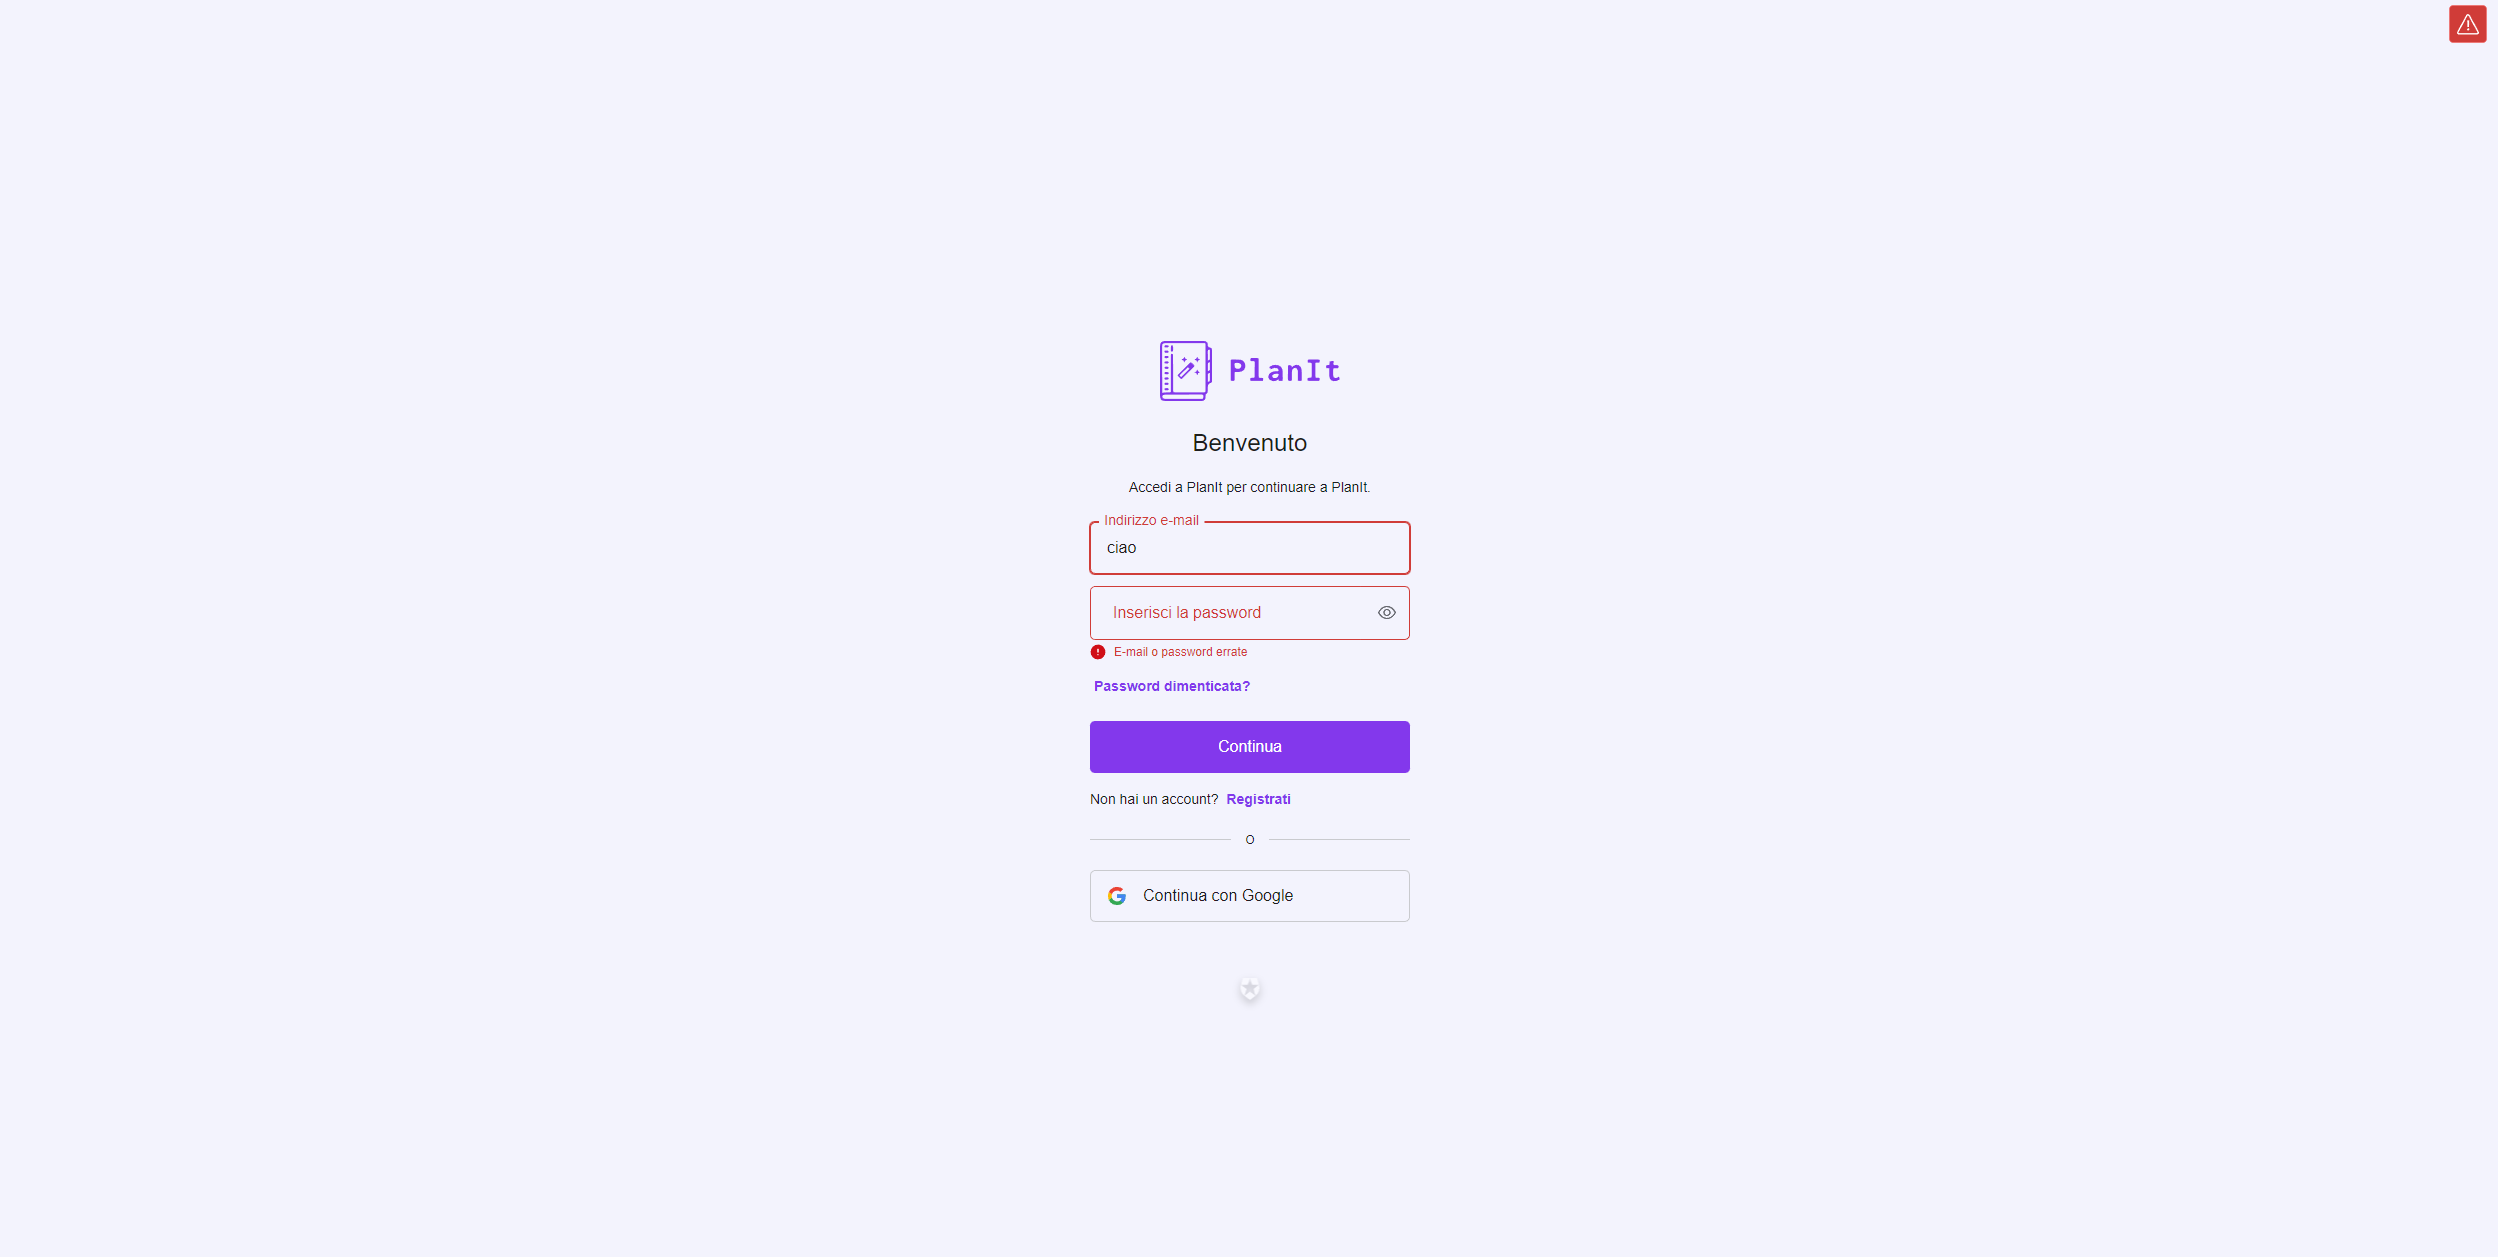
\includegraphics[width=1\textwidth, height=0.3\textheight]{img/png/FrontEnd/Homepage_Autenticazione/login_errato.png}
    \captionof{figure}{FrontEnd - Login errato}
    \blfootnote{Immagine \href{https://github.com/Life-planner/Documentazione/blob/main/D4/img/png/FrontEnd/Homepage_Autenticazione/login_errato.png}{PNG} FrontEnd - Login errato}
\end{center}

Quando l'utente non ha un proprio account PlanIt e non vuole accedere mediante Google, può indirizzarsi alla pagina di registrazione, mediante la scritta "Registrati". Da questa schermata, l'utente può tornare indietro alla pagina di "Login" nel caso in cui avesse sbagliato, può ancora "continuare con Google" oppure, ovviamente, inserire le proprie credenziali con cui si vuole registrare. Ovviamente, le credenziali da inserire devono rispettare delle restrizioni che sono imposte e che vengono mostrate all'utente.\\
Una volta inserite delle credenziali che soddisfano tali restrizioni, l'utente può terminare la procedura di registrazione premendo il tasto "Continua", che lo indirizza alla pagina "Inserimento soprannome". Contemporaneamente, l'utente riceve anche una email per la validazione dell'email inserita per la registrazione; questa validazione è davvero importante, in quanto l'email verificata è quella che si dovrà utilizzare in caso di reset password.

\begin{center}
    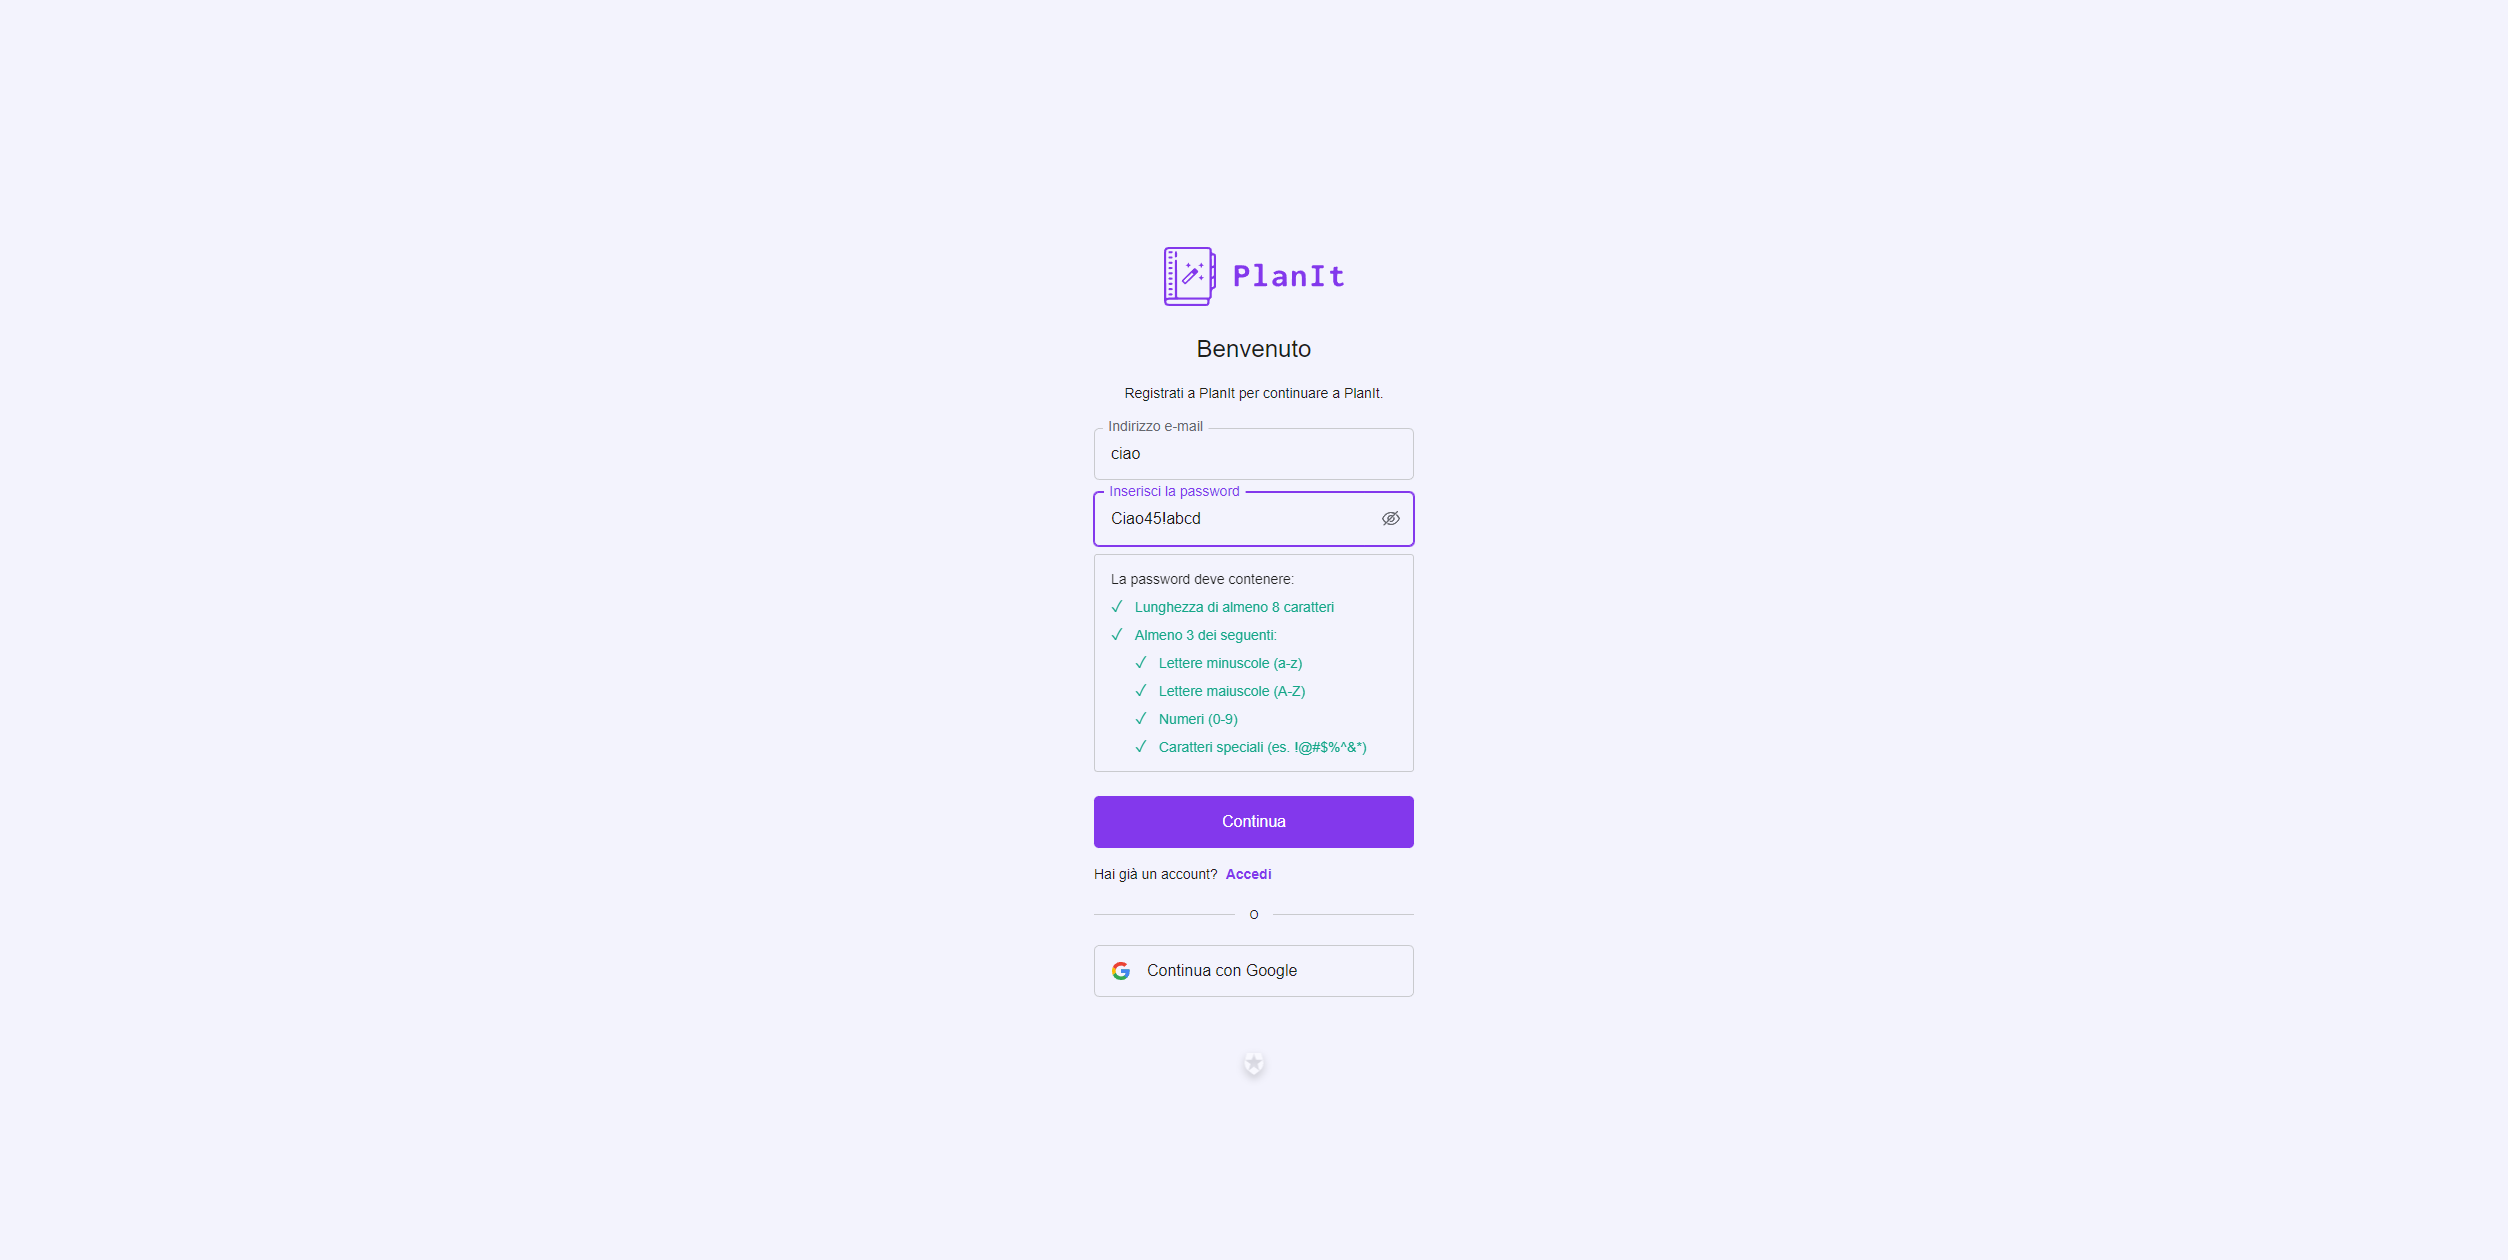
\includegraphics[width=1\textwidth, height=0.3\textheight]{img/png/FrontEnd/Homepage_Autenticazione/registrazione_valida.png}
    \captionof{figure}{FrontEnd - Registrazione valida, segue le restrizioni che vengono imposte e mostrate}
    \blfootnote{Immagine \href{https://github.com/Life-planner/Documentazione/blob/main/D4/img/png/FrontEnd/Homepage_Autenticazione/registrazione_valida.png}{PNG} FrontEnd - Registrazione valida, segue le restrizioni che vengono imposte e mostrate}
\end{center}

Nel caso in cui l'utente si fosse dimenticato la propria password, può schiacciare sulla scritta "Password dimenticata" dalla pagina "Login", che indirizza l'utente alla pagina d'inserimento dell'email con cui si è fatta la registrazione al sito. Il sistema automaticamente invierà un'email di recupero e reset password all'indirizzo email indicato. \\
E' da sottolineare che questa procedura di recupero password, è disponibile solo per gli utenti che hanno deciso di registrarsi al sito mediante credenziali e non con "Google". \\
Infine, dopo l'inserimento dell'email e averla confermata, l'utente visualizza la schermata di conferma che l'email di recupero password è stata inviata; dunque, bisogna controllare la propria casella di posta. Nel caso in cui non fosse stata ricevuta, si può richiedere l'invio di tale email nuovamente.

\begin{center}
    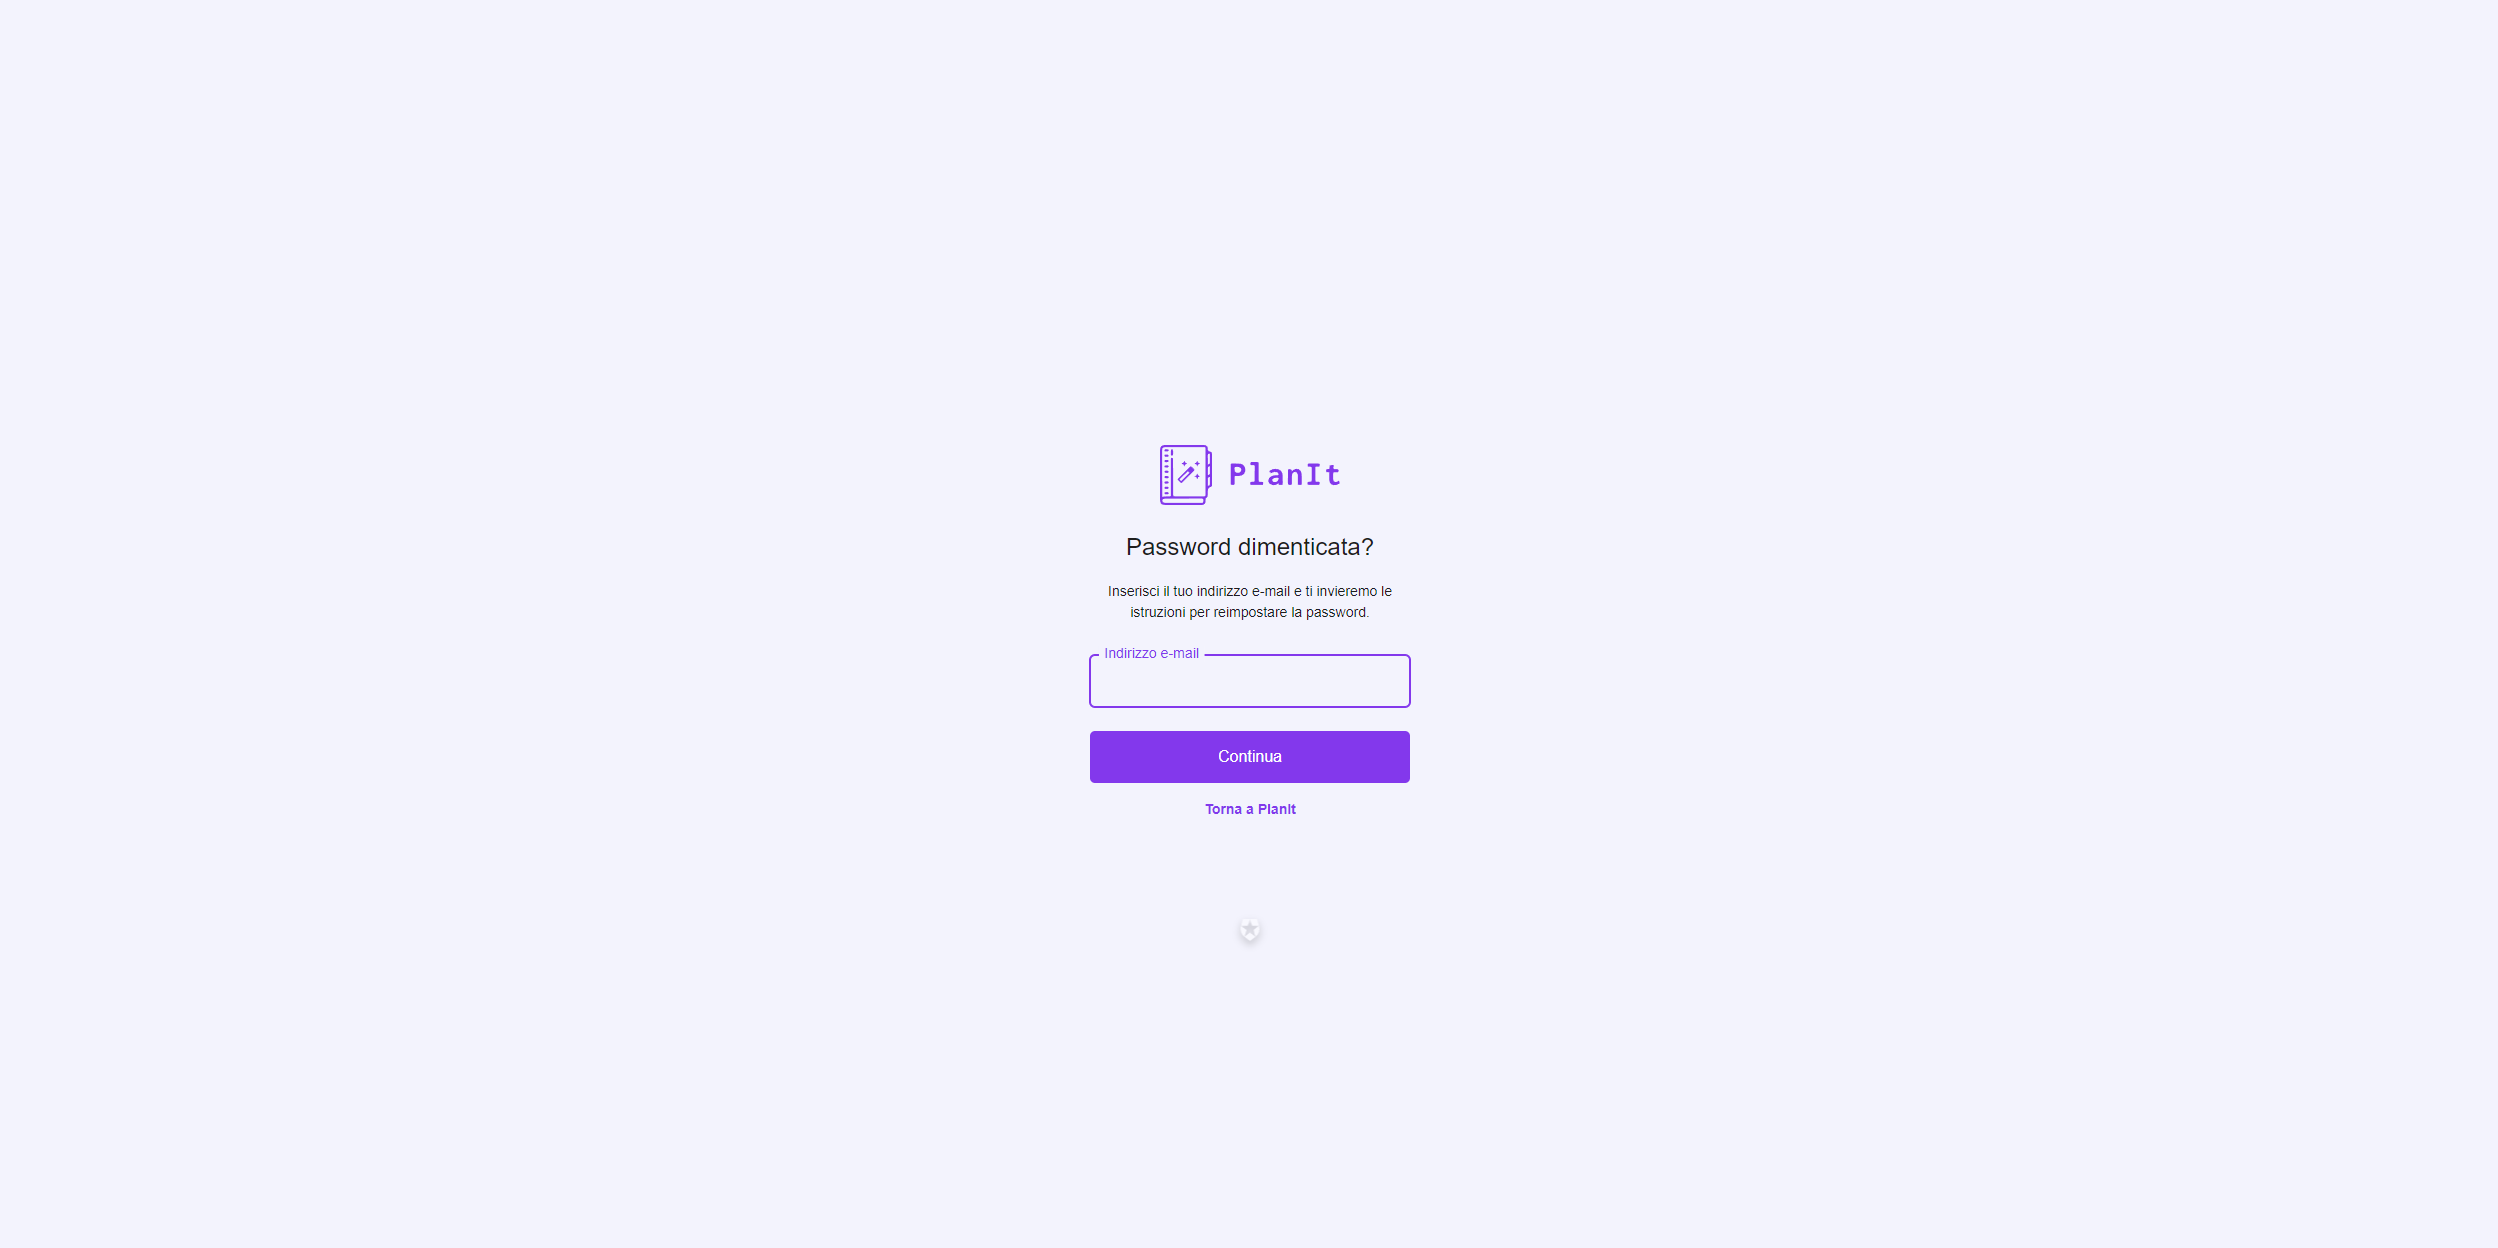
\includegraphics[width=1\textwidth, height=0.3\textheight]{img/png/FrontEnd/Homepage_Autenticazione/recupero_password.png}
    \captionof{figure}{FrontEnd - Recupero password}
    \blfootnote{Immagine \href{https://github.com/Life-planner/Documentazione/blob/main/D4/img/png/FrontEnd/Homepage_Autenticazione/recupero_password.png}{PNG} FrontEnd - Recupero password}
\end{center}

\begin{center}
    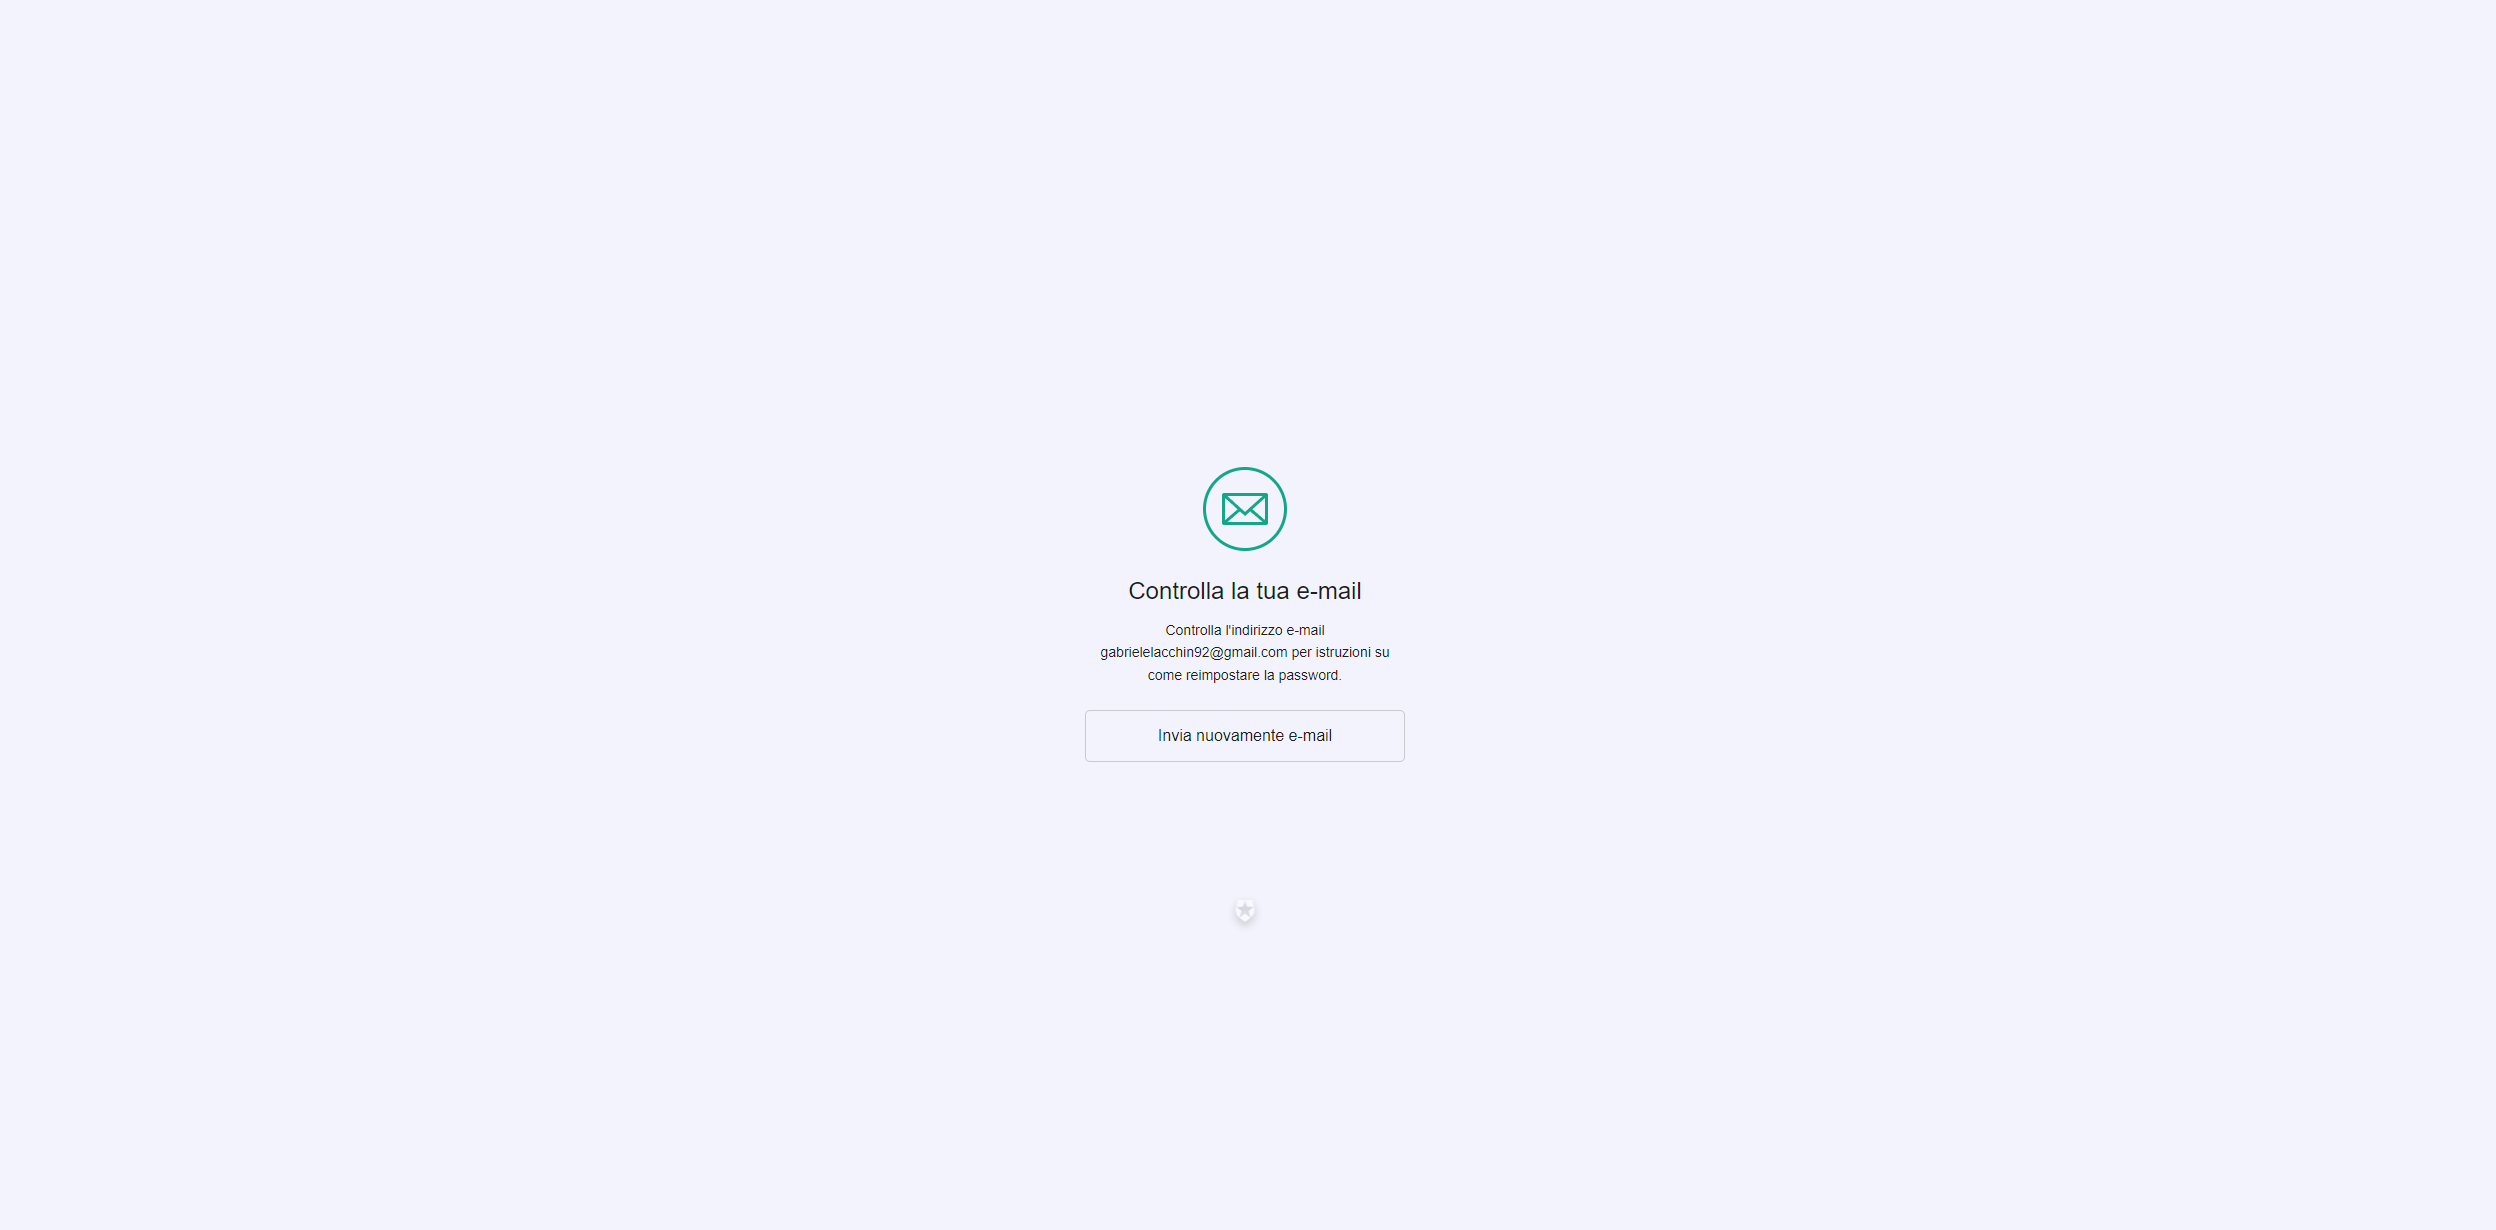
\includegraphics[width=1\textwidth, height=0.3\textheight]{img/png/FrontEnd/Homepage_Autenticazione/controlla_email.png}
    \captionof{figure}{FrontEnd - Controlla email}
    \blfootnote{Immagine \href{https://github.com/Life-planner/Documentazione/blob/main/D4/img/png/FrontEnd/Homepage_Autenticazione/controlla_email.png}{PNG} FrontEnd - Controlla email}
\end{center}

La prima volta che si accede al sito, ovvero dopo la registrazione. Prima di visualizzare la pagina "Calendario" si visualizza la pagina "Inserimento soprannome", dove l'utente può definire un soprannome, che nel caso in cui non fosse inserito, rimane l'email. Infatti, nel caso in cui l'utente volesse inserire un soprannome, può scriverlo e schiacciare su "Continua". Invece, nel caso in cui non gli interessasse, può schiacciare direttamente su "salta" e sarà indirizzato immediatamente alla pagina "Calendario".

\begin{center}
    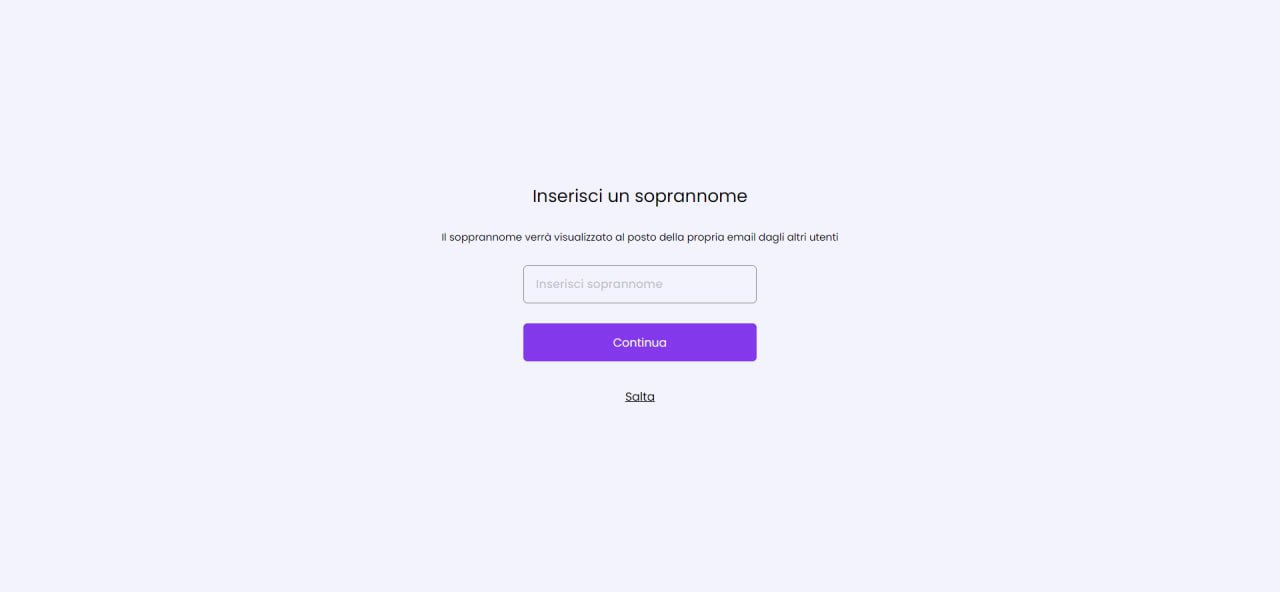
\includegraphics[width=1\textwidth, height=0.3\textheight]{img/png/FrontEnd/InserimentoSoprannome.jpg}
    \captionof{figure}{FrontEnd - Inserimento soprannome}
    \blfootnote{Immagine \href{https://github.com/Life-planner/Documentazione/blob/main/D4/img/png/FrontEnd/InserimentoSoprannome.jpg}{PNG} FrontEnd - Inserimento soprannome}
\end{center}

Dopo aver fatto l'autenticazione e se non è la prima volta che si accede al sito (in quel caso prima della pagina "Calendario", come detto precedentemente, si visualizza la pagina "Inserimento soprannome"), l'utente autenticato visualizza la pagina "Calendario", da cui può passare a tutte le altre pagine (ricordiamo che oltre a "Calendario" è stata sviluppata solo la pagina "Eventi" in questo protitipo), può creare un evento  e/o calendario, possibilità visualizzabile dopo aver premuto il "+" in baso a destra, può visualizzare la lista di calendari personali, e anche quelli condivisi, dal bottone "Calendari", che apre una side-bar in cui si possono selezionare i calendari da visualizzare nella schermata "Calendario, e infine può spostarsi temporalmente nel tempo di settimana in settimana grazie ai bottoni "<", con cui si va indietro, e ">", con cui si va avanti, e tornare alla data corrente mediante il bottone "Oggi". Adesso andiamo un po' più nello specifico delle cose visualizzabili e che si possono fare in questa pagina.

\begin{center}
    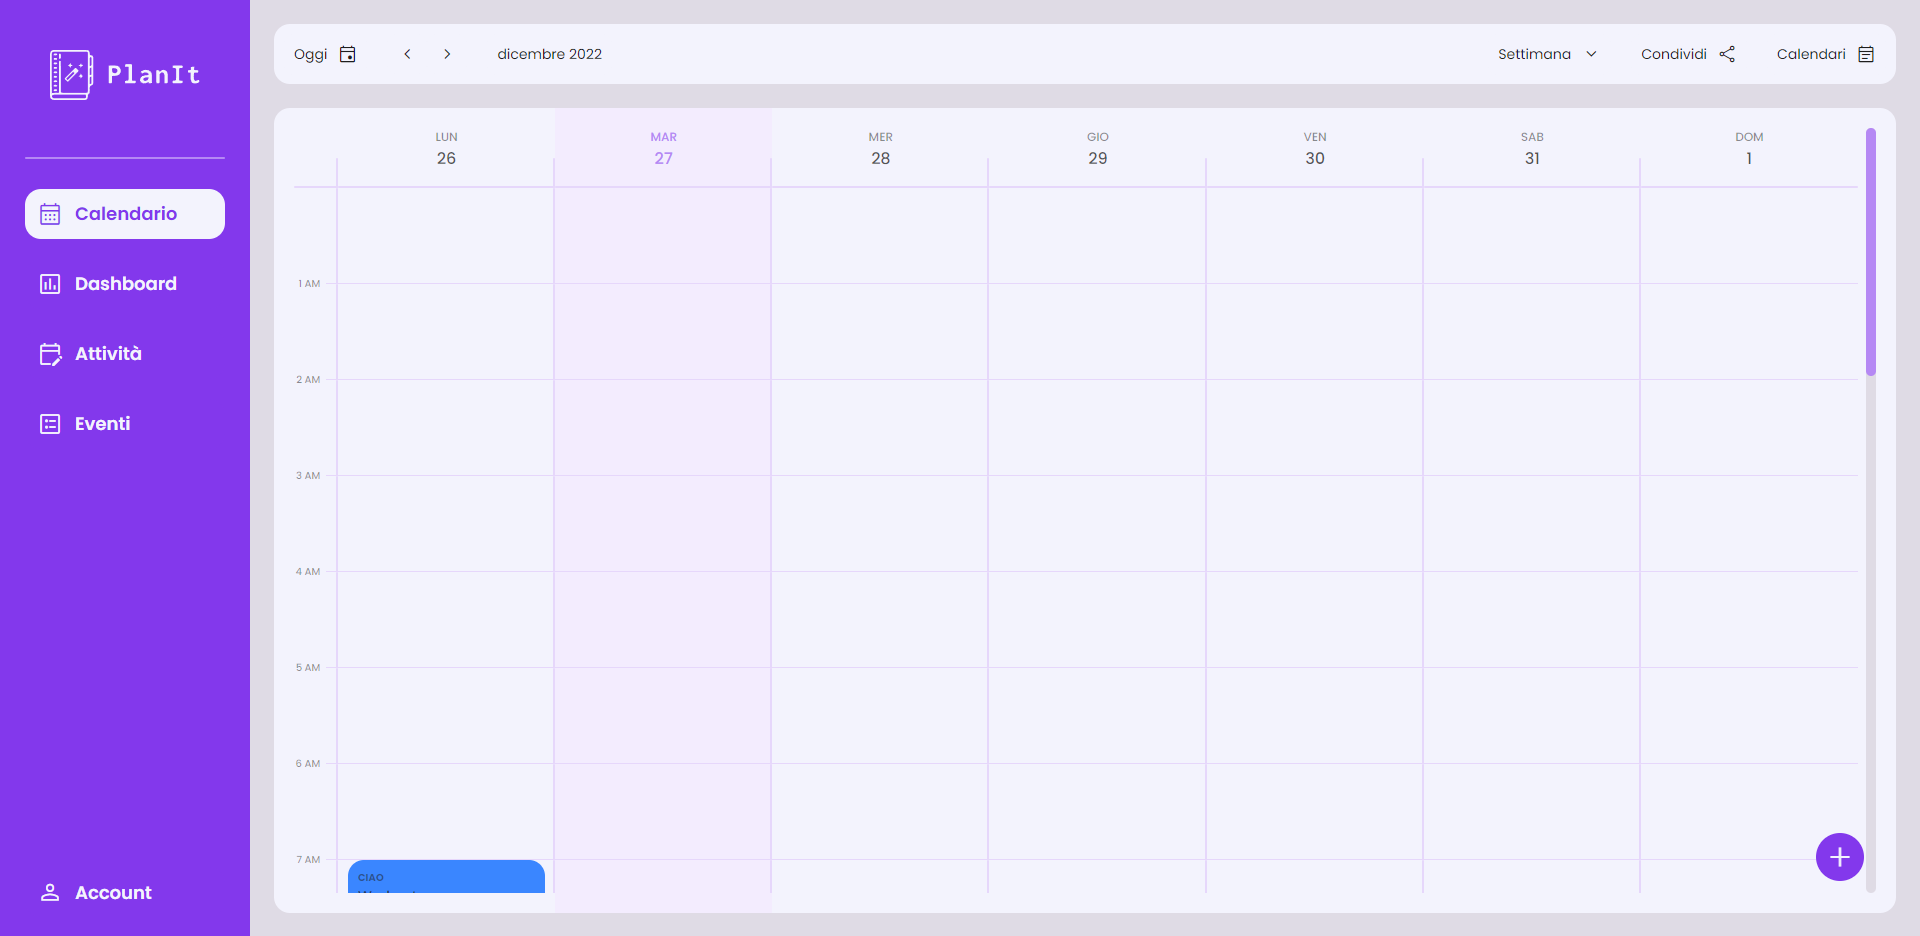
\includegraphics[width=1\textwidth, height=0.3\textheight]{img/png/FrontEnd/Calendario/schermata_calendario.png}
    \captionof{figure}{FrontEnd - schermata "Calendario"}
    \blfootnote{Immagine \href{https://github.com/Life-planner/Documentazione/blob/main/D4/img/png/FrontEnd/Calendario/schermata_calendario.png}{PNG} FrontEnd - schermata "Calendario"}
\end{center}

Dunque, premendo il bottone "Calendari" in alto a destra, appare questa side-bar, mostrata nella foto sottostante, in cui è presente una lista di tutti i calendari appartenenti all'utente. I calendari condivisi sono distinguibili grazie allo stereotipo di due "persone" che si trova a fianco di tali calendari. La funzionalità di questa side-bar, oltre che far visualizzare la lista di calendari personali, è anche quella di permettere all'utente di filtrare, spuntandoli, quale calendari visualizzare, e quindi i rispettivi eventi, nella pagina "Calendario".

\begin{center}
    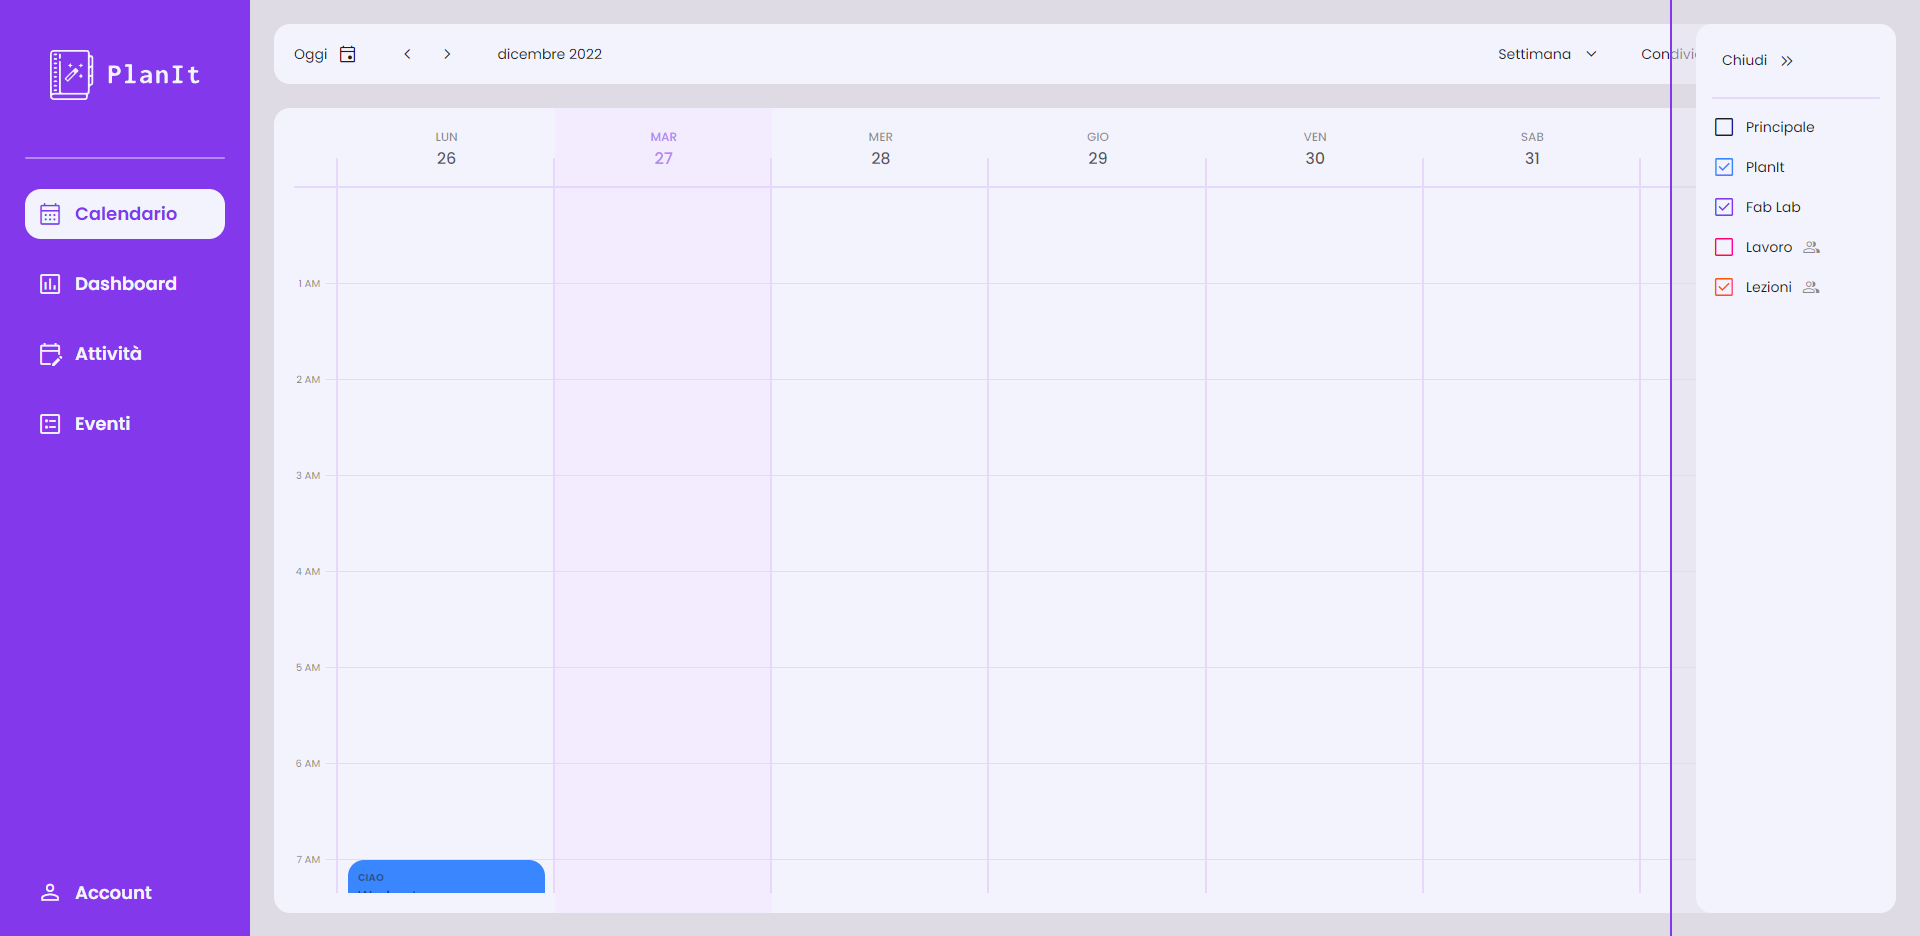
\includegraphics[width=1\textwidth, height=0.3\textheight]{img/png/FrontEnd/Calendario/calendario_calendari.png}
    \captionof{figure}{FrontEnd - side-bar Calendari}
    \blfootnote{Immagine \href{https://github.com/Life-planner/Documentazione/blob/main/D4/img/png/FrontEnd/Calendario/calendario_calendari.png}{PNG} schermata "Calendario" - side-bar Calendari}
\end{center}

Dopo, premendo il tasto "+" in basso a destra è possibile aprire un fab, dove appare la scritta "Evento" e "Calendario". Grazie a questi due scelte, è possibile poter creare un evento singolo
\begin{comment}
, specifichiamo che in questa schermata si può creare solo quello singolo, a differenza della schermata "Eventi" in cui si possono creare anche quelli ripetuti, 
\end{comment}
e/o un calendario. Dunque, premendo una delle tue scelte, appare un pop-up di creazione calendario o evento.

\begin{center}
    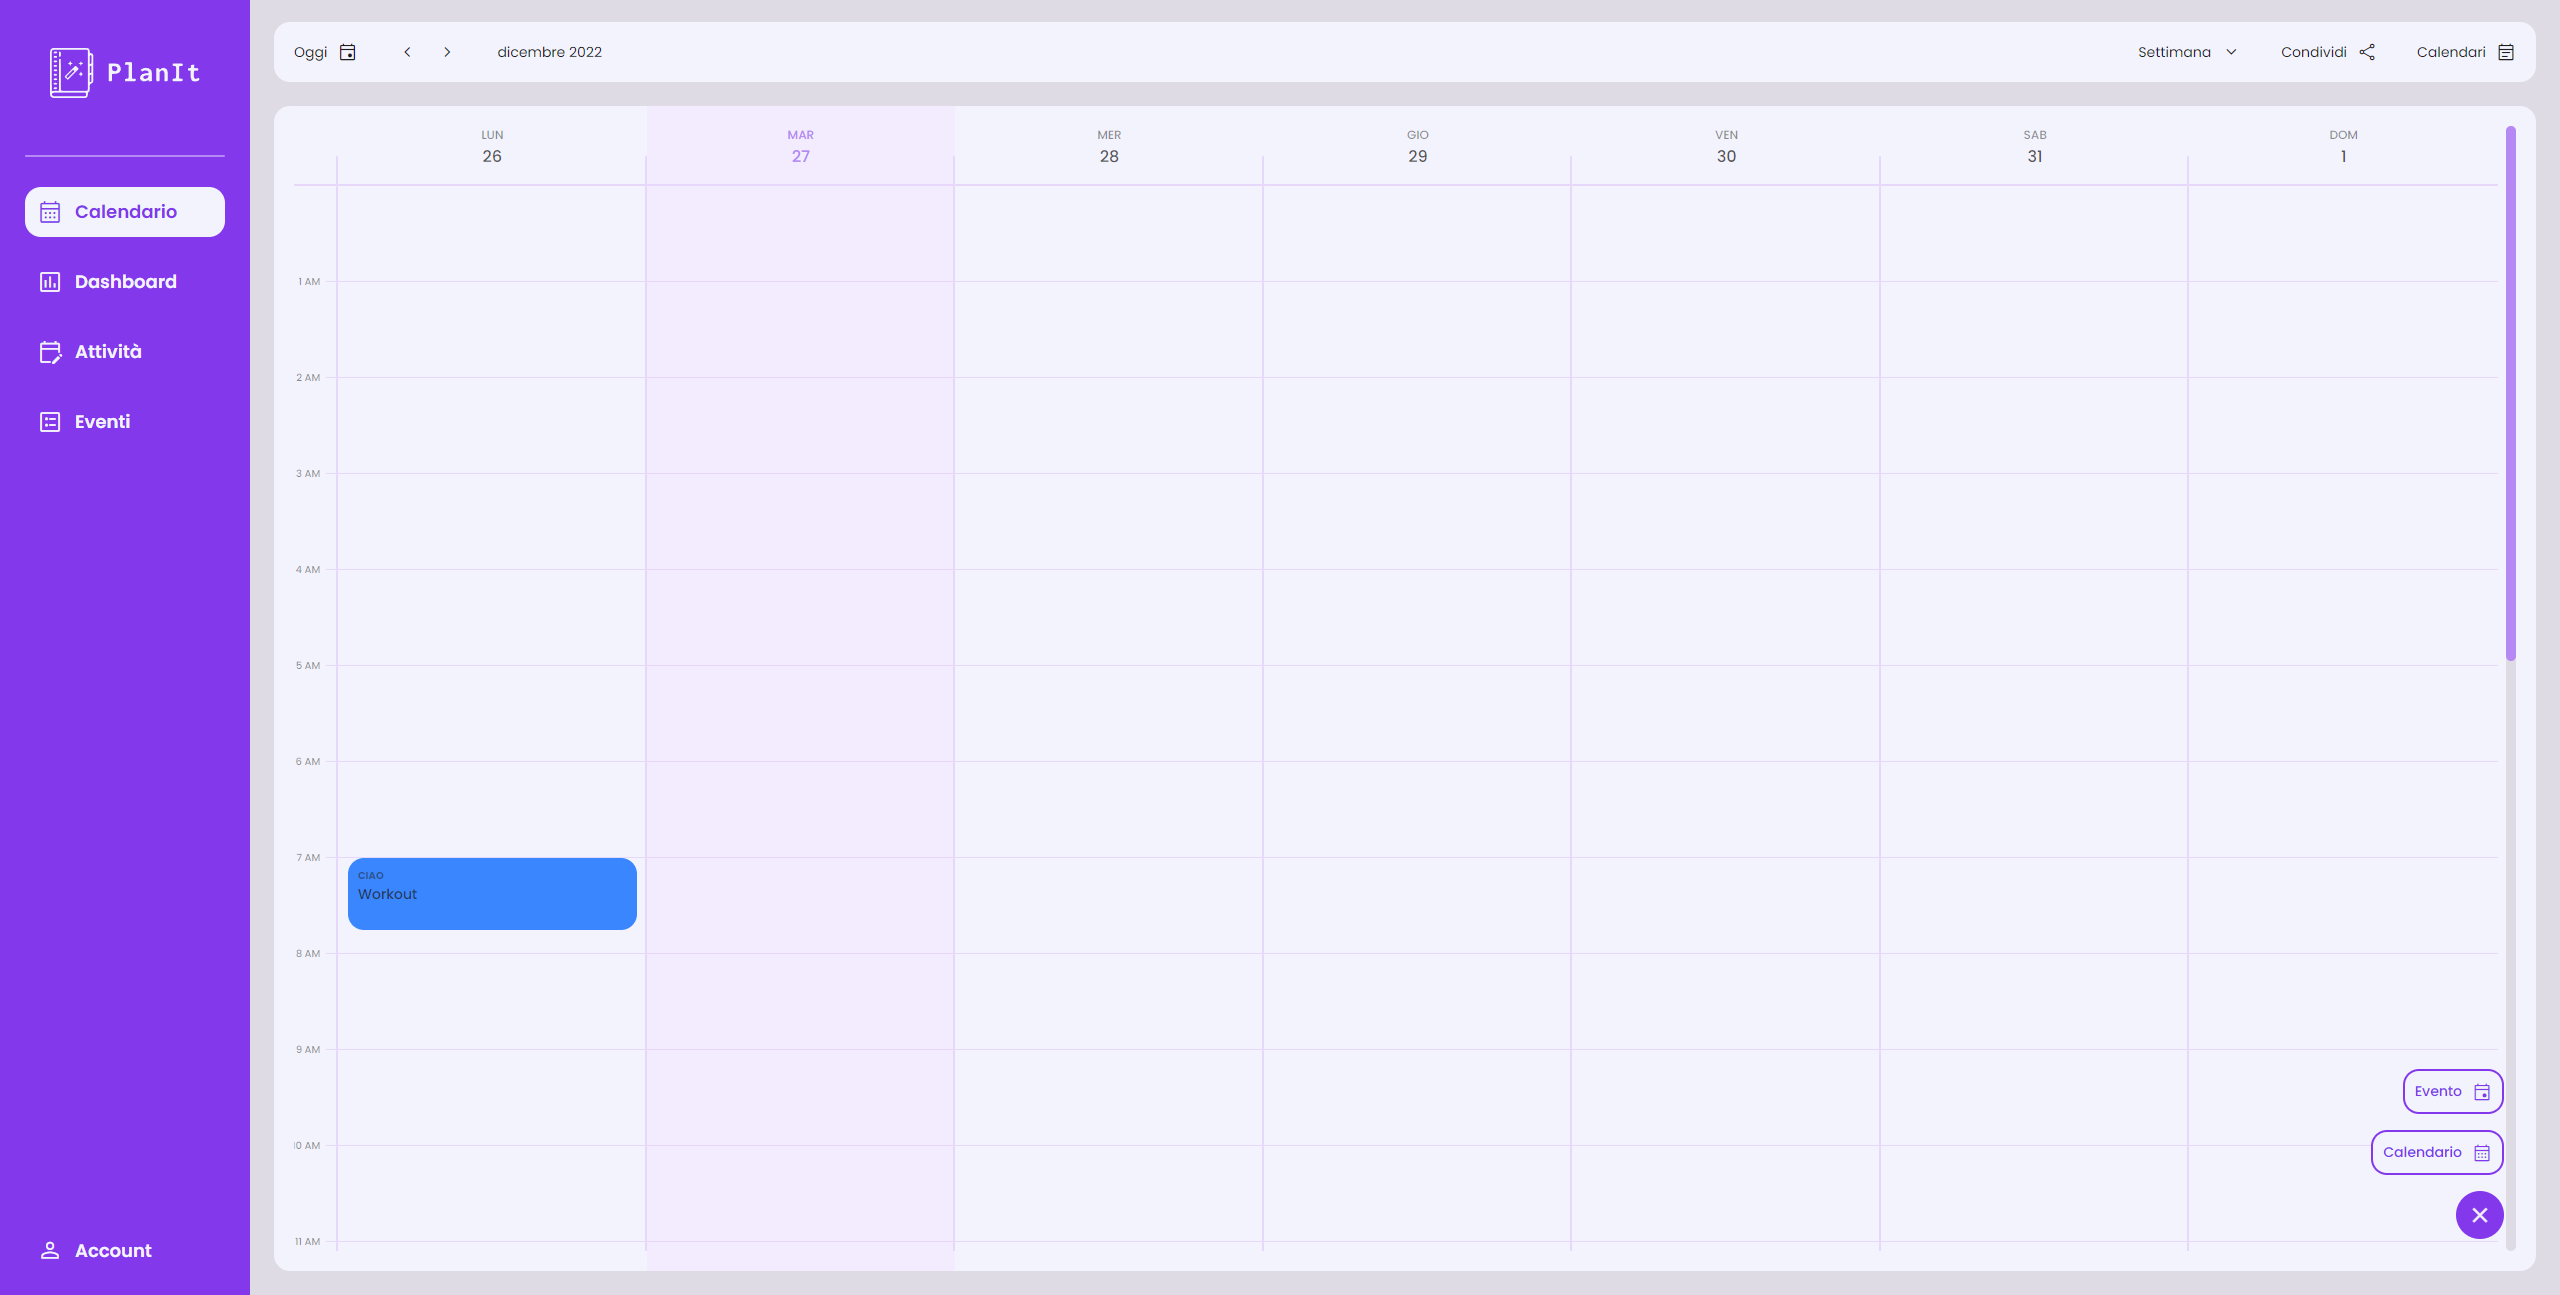
\includegraphics[width=1\textwidth, height=0.3\textheight]{img/png/FrontEnd/Calendario/calendario_creazione.png}
    \captionof{figure}{FrontEnd - Scelta creazione}
    \blfootnote{Immagine \href{https://github.com/Life-planner/Documentazione/blob/main/D4/img/png/FrontEnd/Calendario/calendario_creazione.png}{PNG} schermata "Calendario" - Scelta creazione}
\end{center}

Il pop-up sottostante è quello di "Crea Calendario". Tutti i campi visualizzabili sono compilabili, eccetto per "Luogo", in quanto non abbiamo sviluppato la possibilità dell'utente d'indicare il luogo dove si tiene un evento. Dopo aver compilato a piacere i vari campi, l'utente ha la possibilità di salvarlo, oppure anche di annullare l'azione; ricordiamo che il nome del calendario è obbligatorio per poter creare un calendario e quindi far andare a buon fine il salvataggio di quest'ultimo.

\begin{center}
    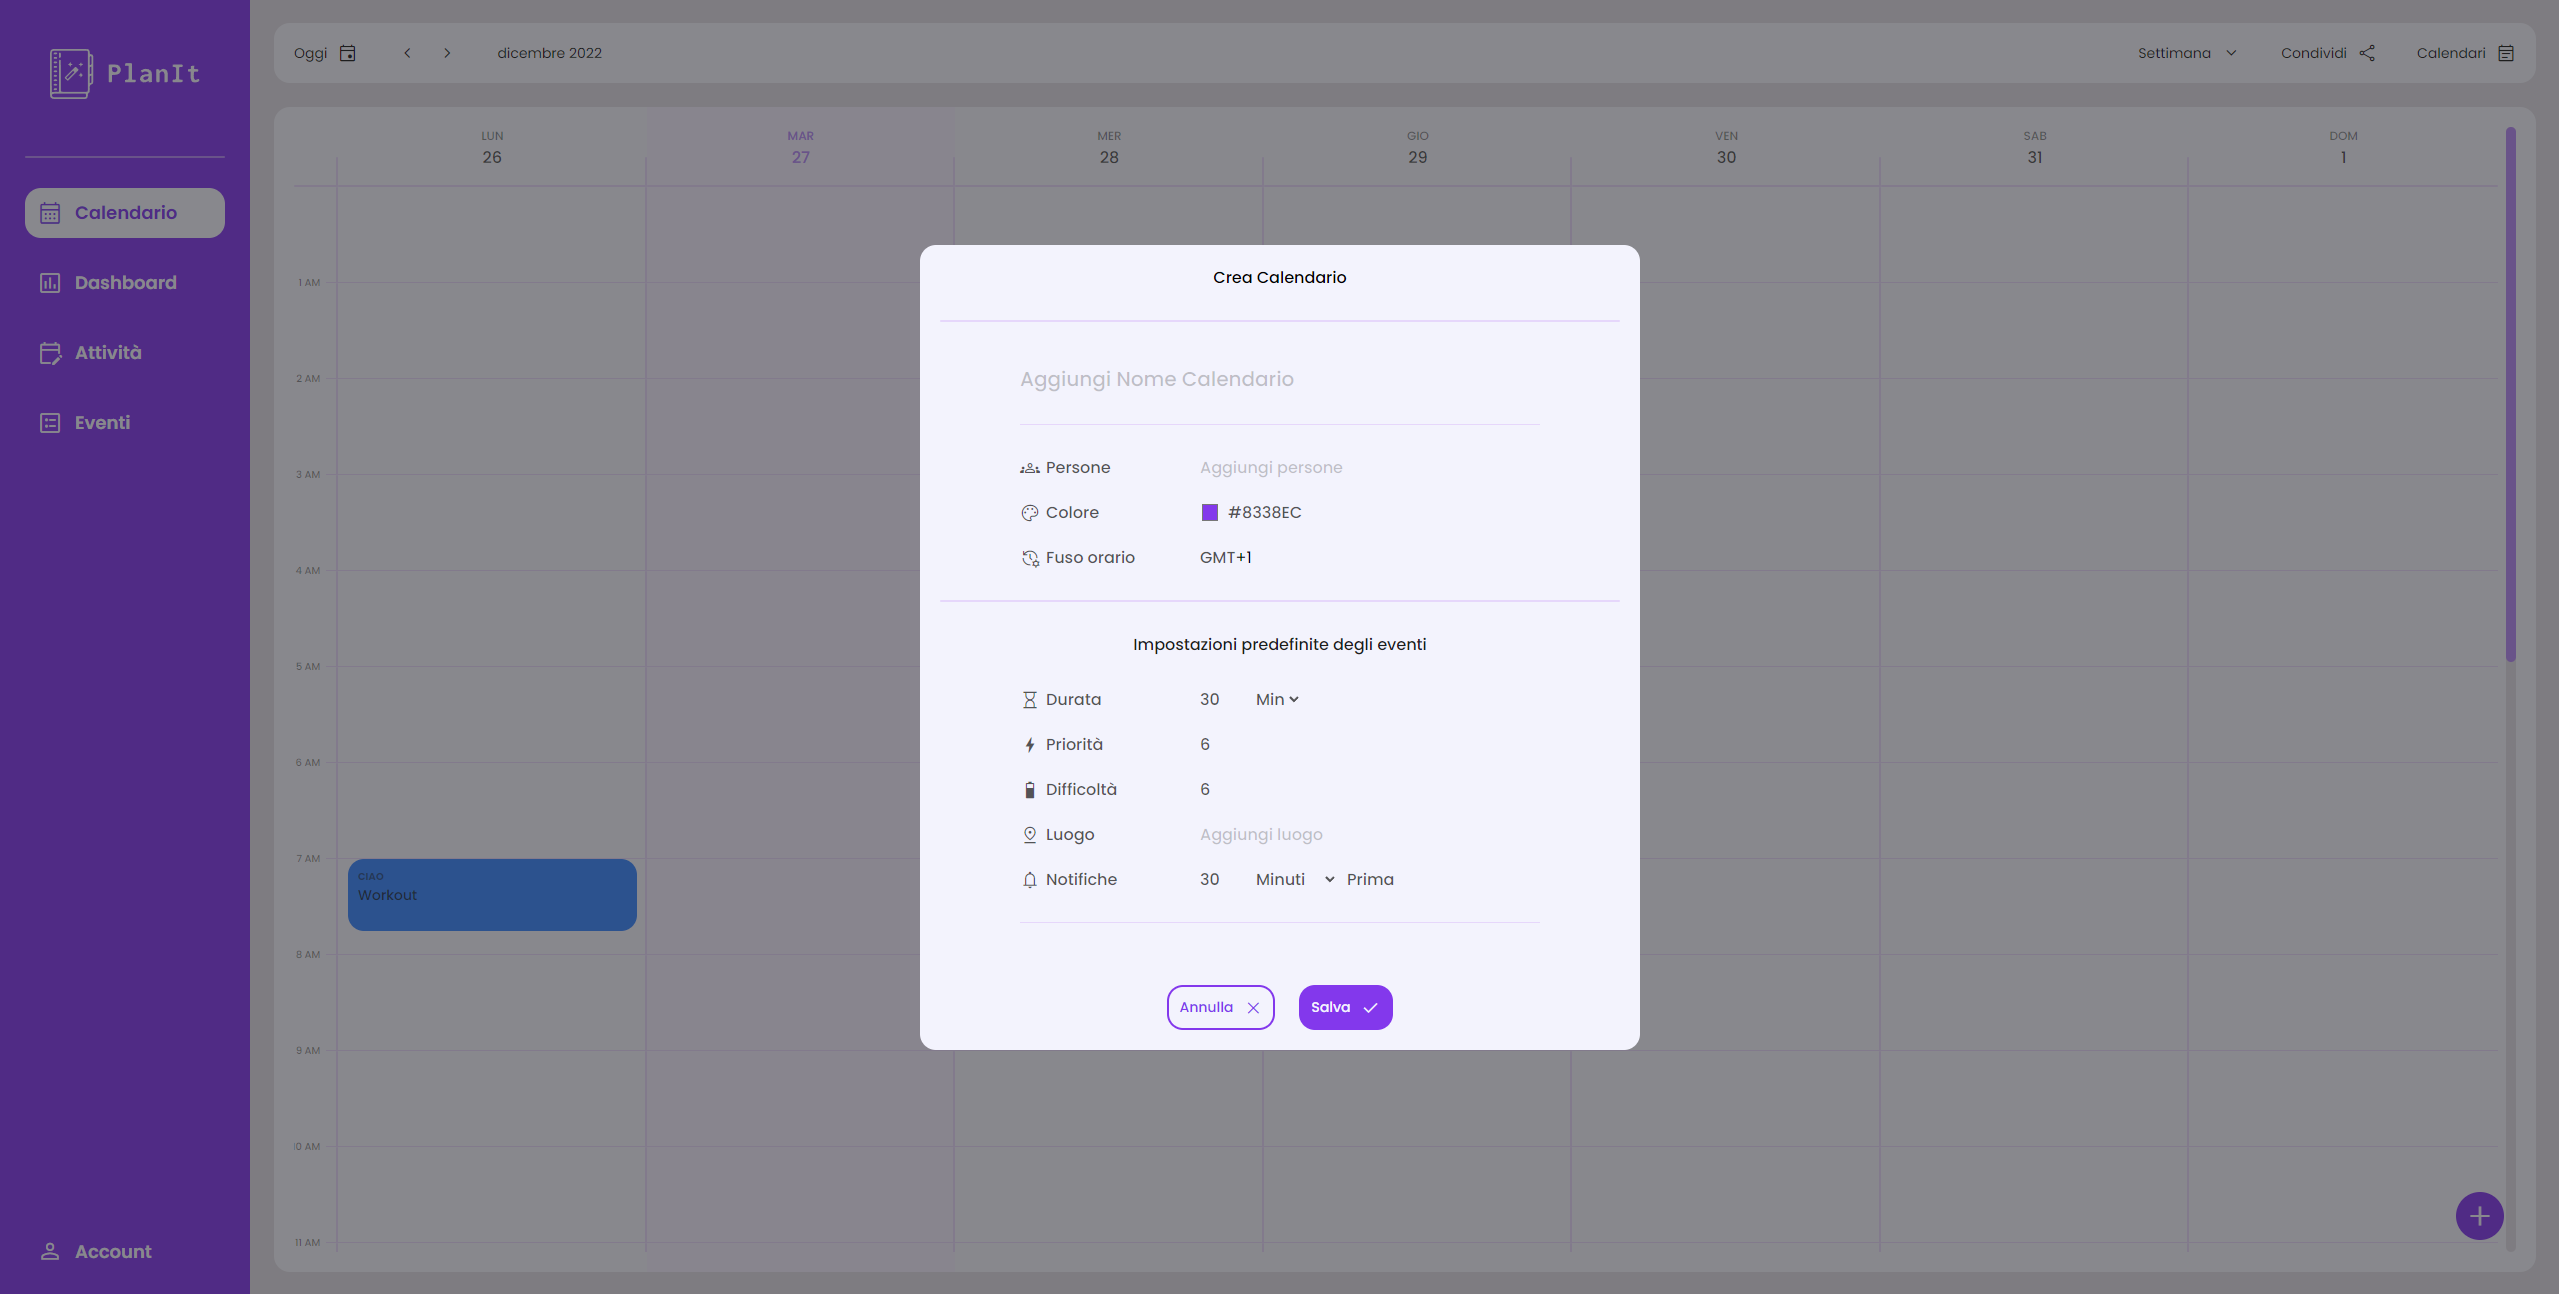
\includegraphics[width=1\textwidth, height=0.3\textheight]{img/png/FrontEnd/Calendario/calendario_creaCalendario.png}
    \captionof{figure}{FrontEnd - Crea Calendario}
    \blfootnote{Immagine \href{https://github.com/Life-planner/Documentazione/blob/main/D4/img/png/FrontEnd/Calendario/calendario_creaCalendario.png}{PNG} schermata "Calendario" - Crea Calendario}
\end{center}

Invece, il pop-up sottostante è quello che si ottiene quando l'utente vuole creare un evento. Tutti i campi sono compilabili, eccetto per il campo "Luogo", come già detto per "Crea Calendario". Dopo aver compilato a piacere i vari campi (ricordiamo, che il titolo dell'evento e la sua data devono essere definiti obbligatoriamente per poter creare un evento) l'utente ha la possibilità di salvarlo, oppure anche di annullare l'azione.

\begin{center}
    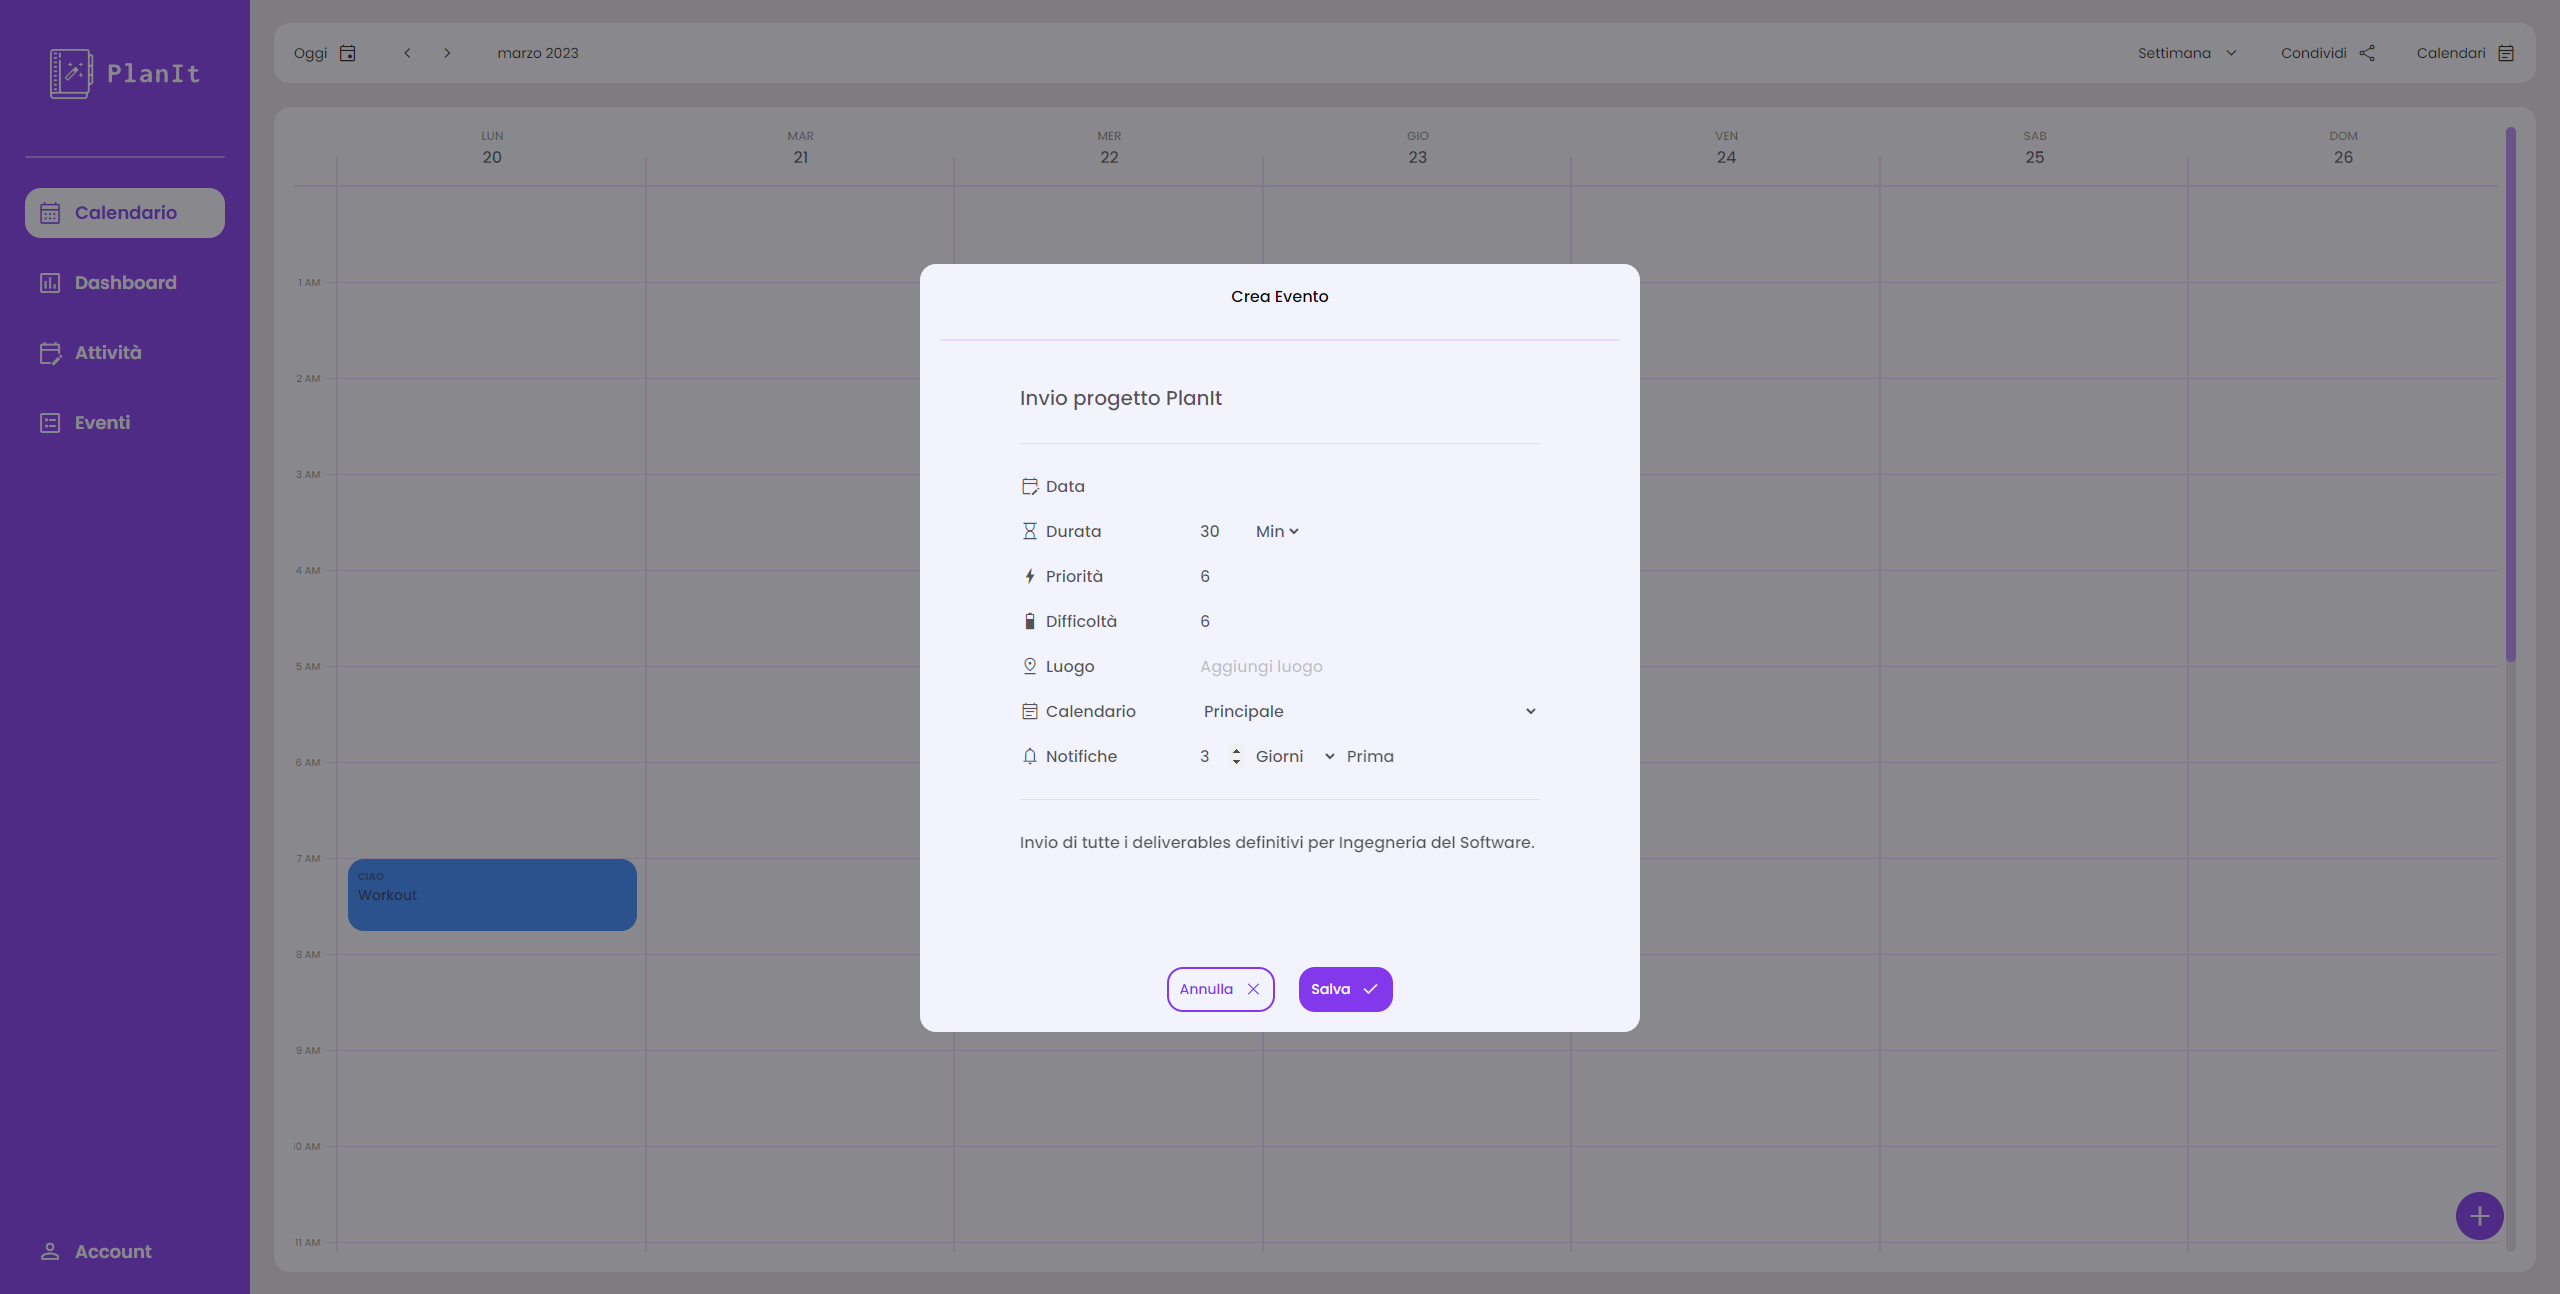
\includegraphics[width=1\textwidth, height=0.3\textheight]{img/png/FrontEnd/Calendario/calendario_creaEvento.png}
    \captionof{figure}{FrontEnd - Crea Evento}
    \blfootnote{Immagine \href{https://github.com/Life-planner/Documentazione/blob/main/D4/img/png/FrontEnd/Calendario/calendario_creaEvento.png}{PNG} schermata "Calendario" - Crea Evento}
\end{center}

Come già detto in precedenza, mediante i bottoni "<", ">" e "Oggi" l'utente può rispettivamente:
\begin{itemize}
    \item andare indietro di una settimana alla volta nel calendario; si guardi la prima immagine sottostante a questa lista;
    \item andare avanti di una settimana alla volta nel calendario; si guardi la seconda immagine sottostante a questa lista;
    \item tornare alla settimana presente.
\end{itemize}


\begin{center}
    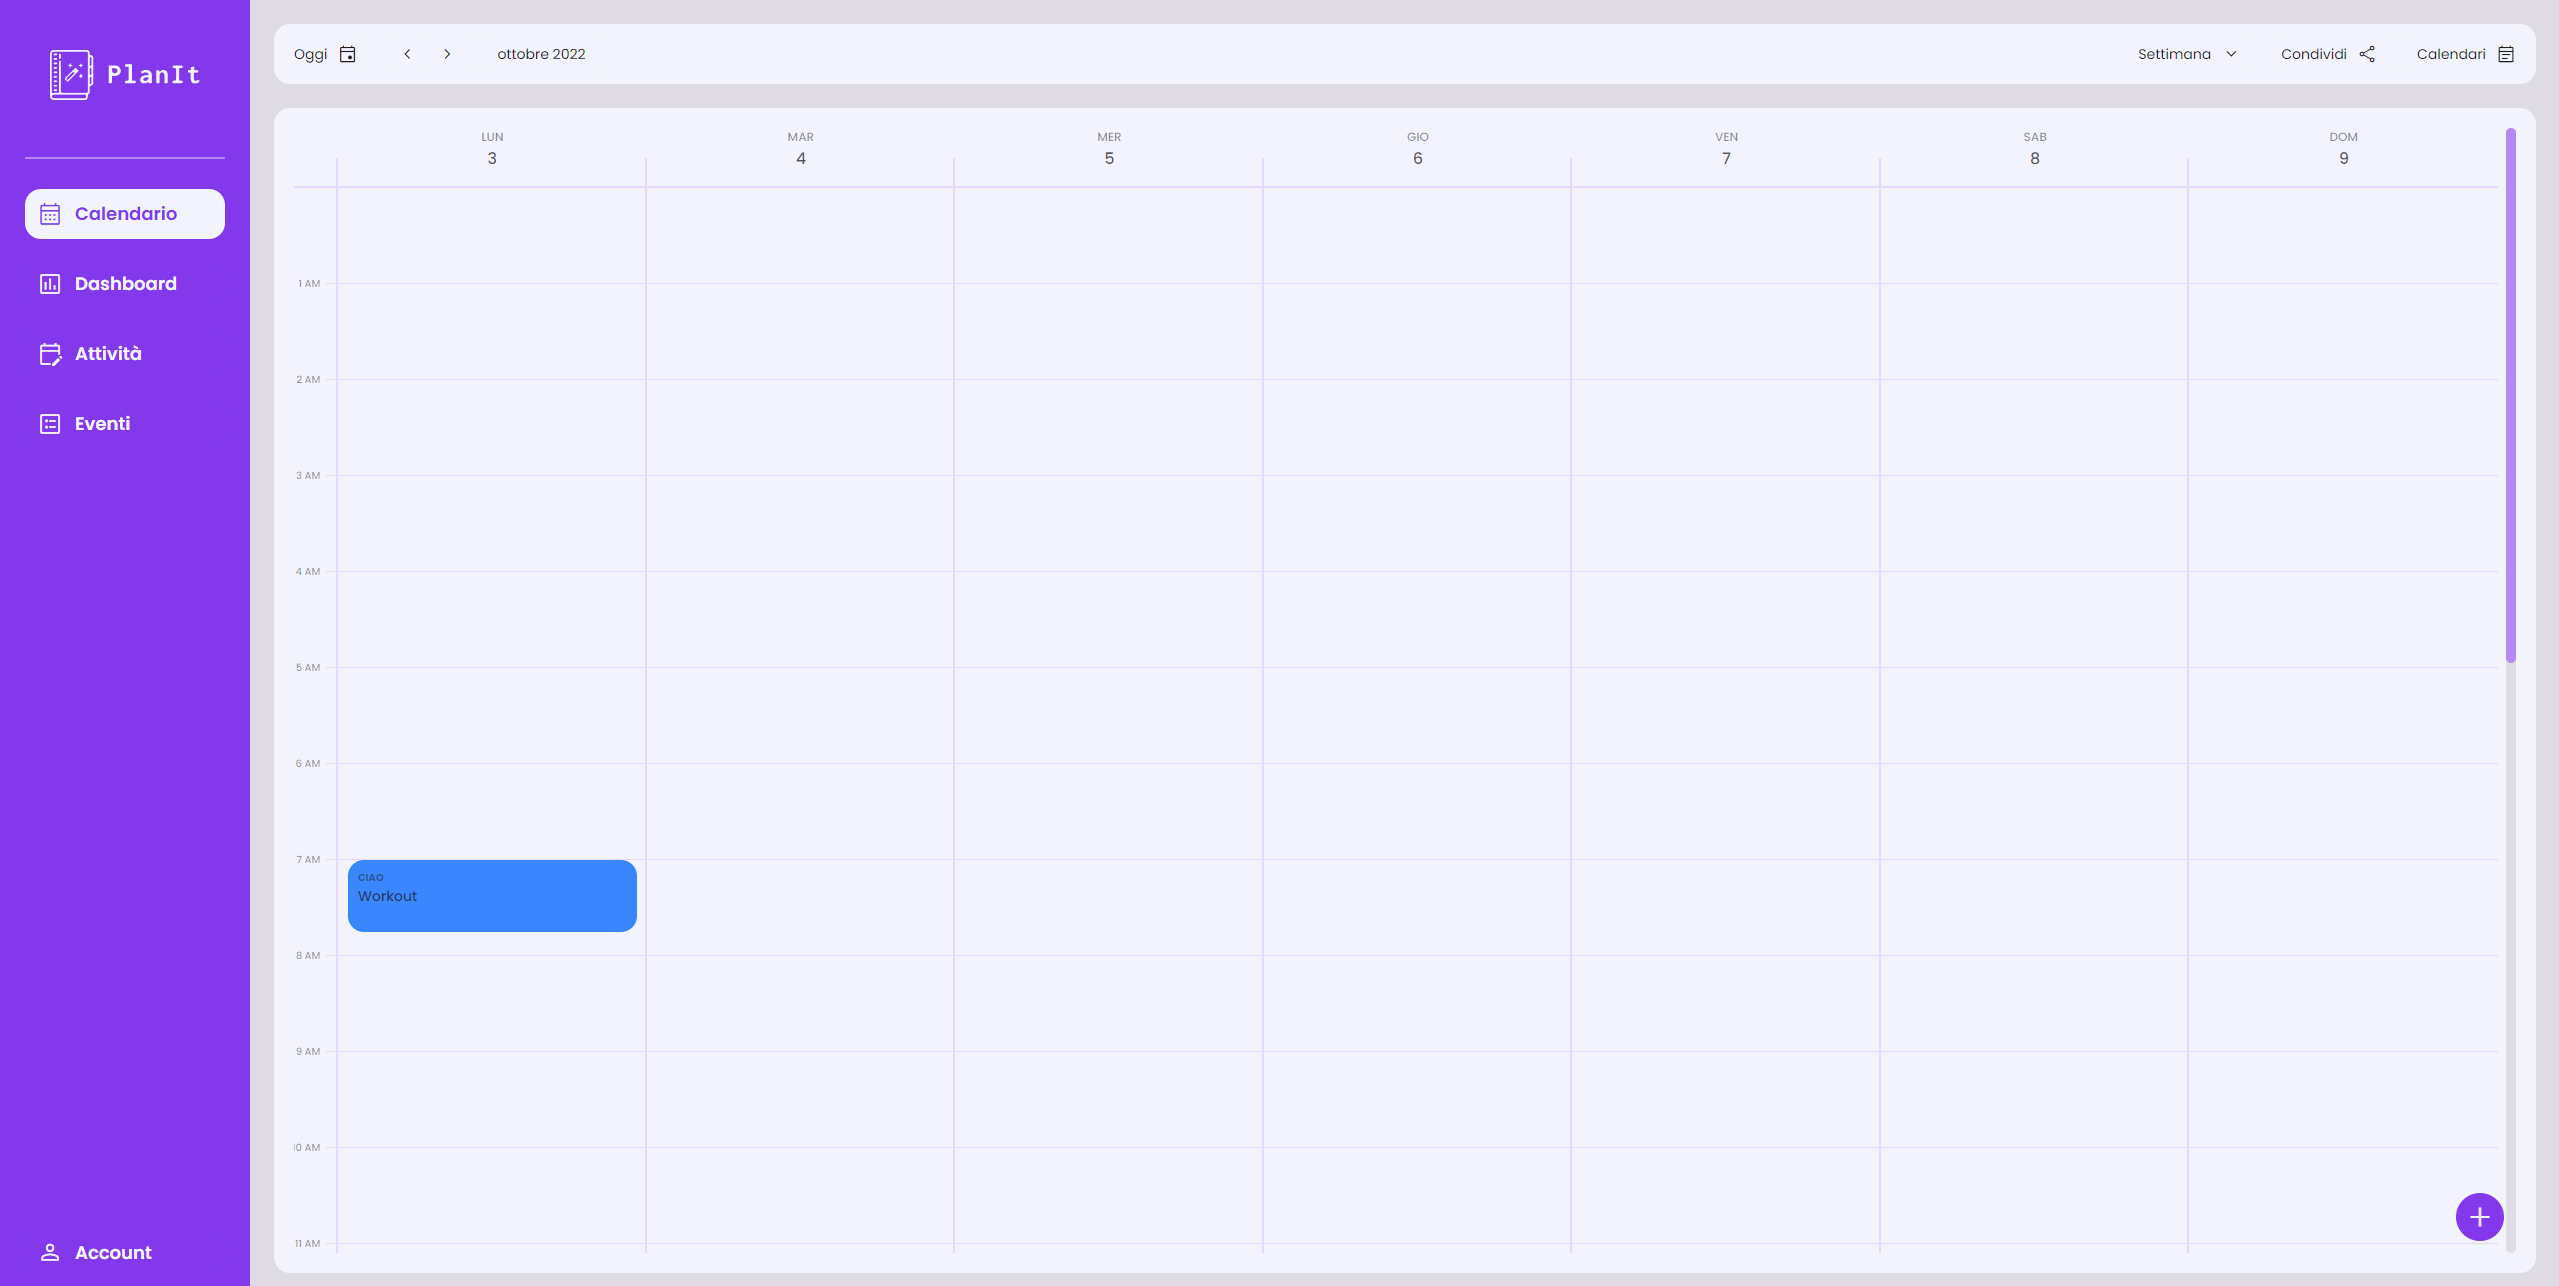
\includegraphics[width=1\textwidth, height=0.3\textheight]{img/png/FrontEnd/Calendario/calendario_passato.png}
    \captionof{figure}{FrontEnd - Andare indietro di settimane}
    \blfootnote{Immagine \href{https://github.com/Life-planner/Documentazione/blob/main/D4/img/png/FrontEnd/Calendario/calendario_passato.png}{PNG} schermata "Calendario" - Andare indietro di settimane}
\end{center}

\begin{center}
    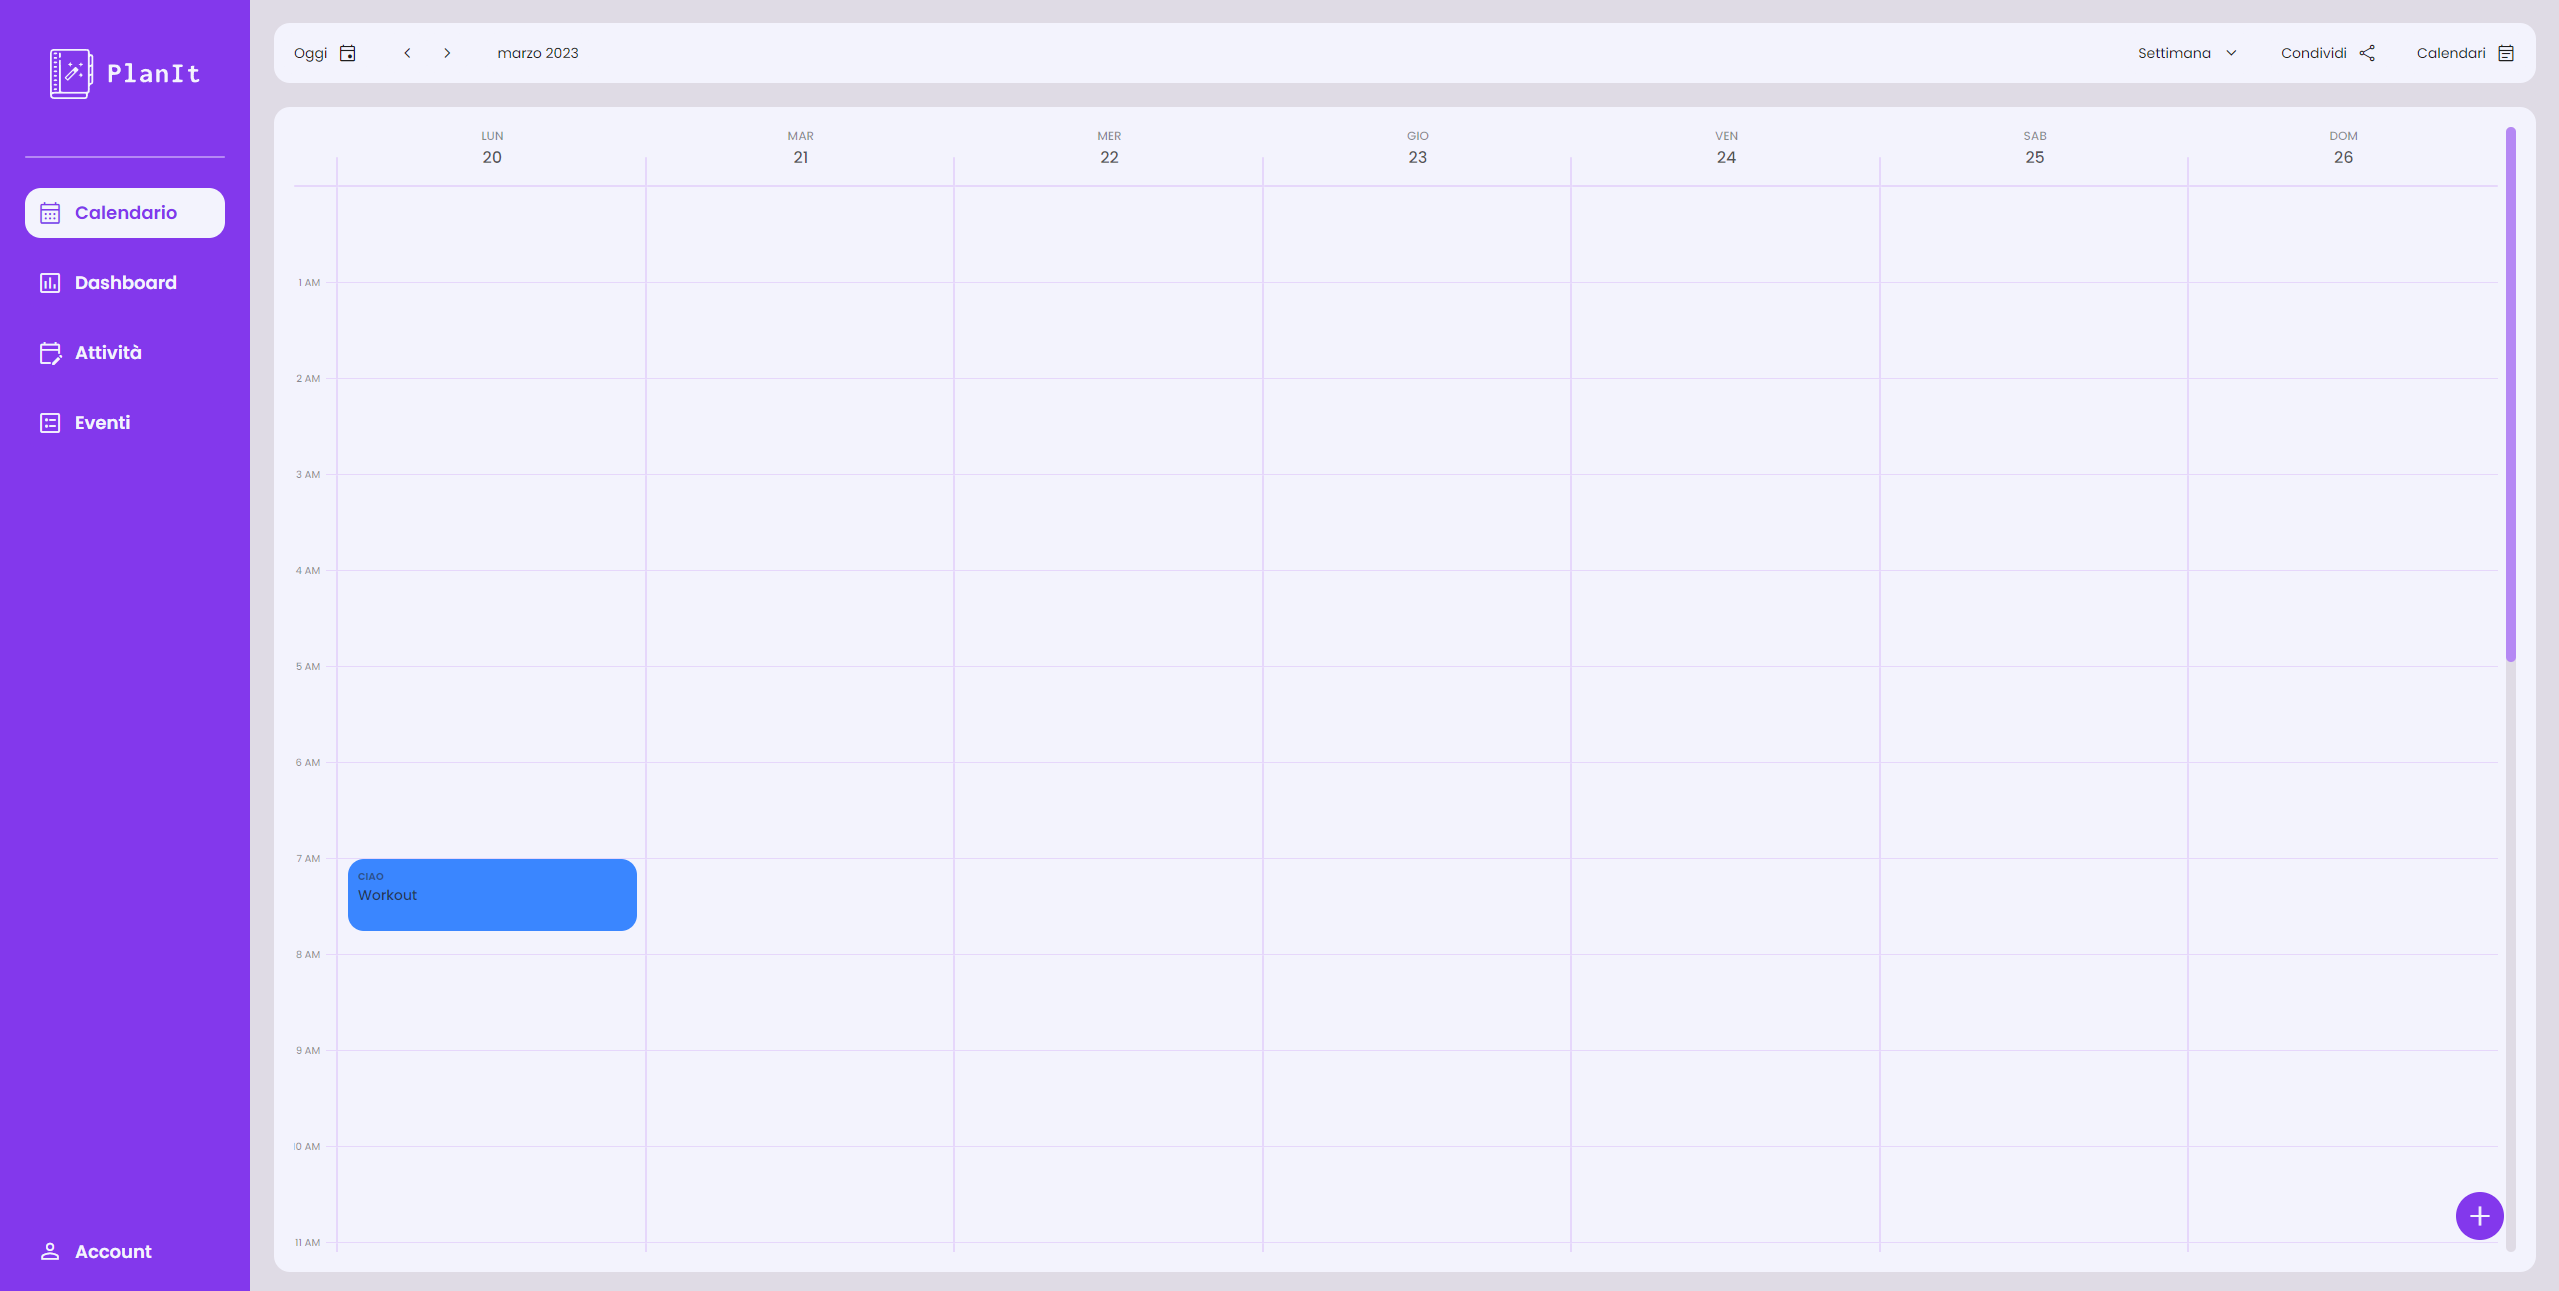
\includegraphics[width=1\textwidth, height=0.3\textheight]{img/png/FrontEnd/Calendario/calendario_futuro.png}
    \captionof{figure}{FrontEnd - Andare avanti di settimane}
    \blfootnote{Immagine \href{https://github.com/Life-planner/Documentazione/blob/main/D4/img/png/FrontEnd/Calendario/calendario_futuro.png}{PNG} schermata "Calendario" - Andare avanti di settimane}
\end{center}

Dalla schermata "Calendario", come citato precedentemente, l'utente autenticato può passare alla schermata "Eventi". Da quest'ultima schermata, oltre a poter creare nuovi eventi singoli e nuovi calendari, mediante gli stessi pop-up ottenibili nella pagina "Calendario", è possibile anche modificare sia gli eventi che i calendari salvati. Adesso andiamo più nello specifico di ciò che può visualizzare e fare l'utente da questa schermata.

\begin{center}
    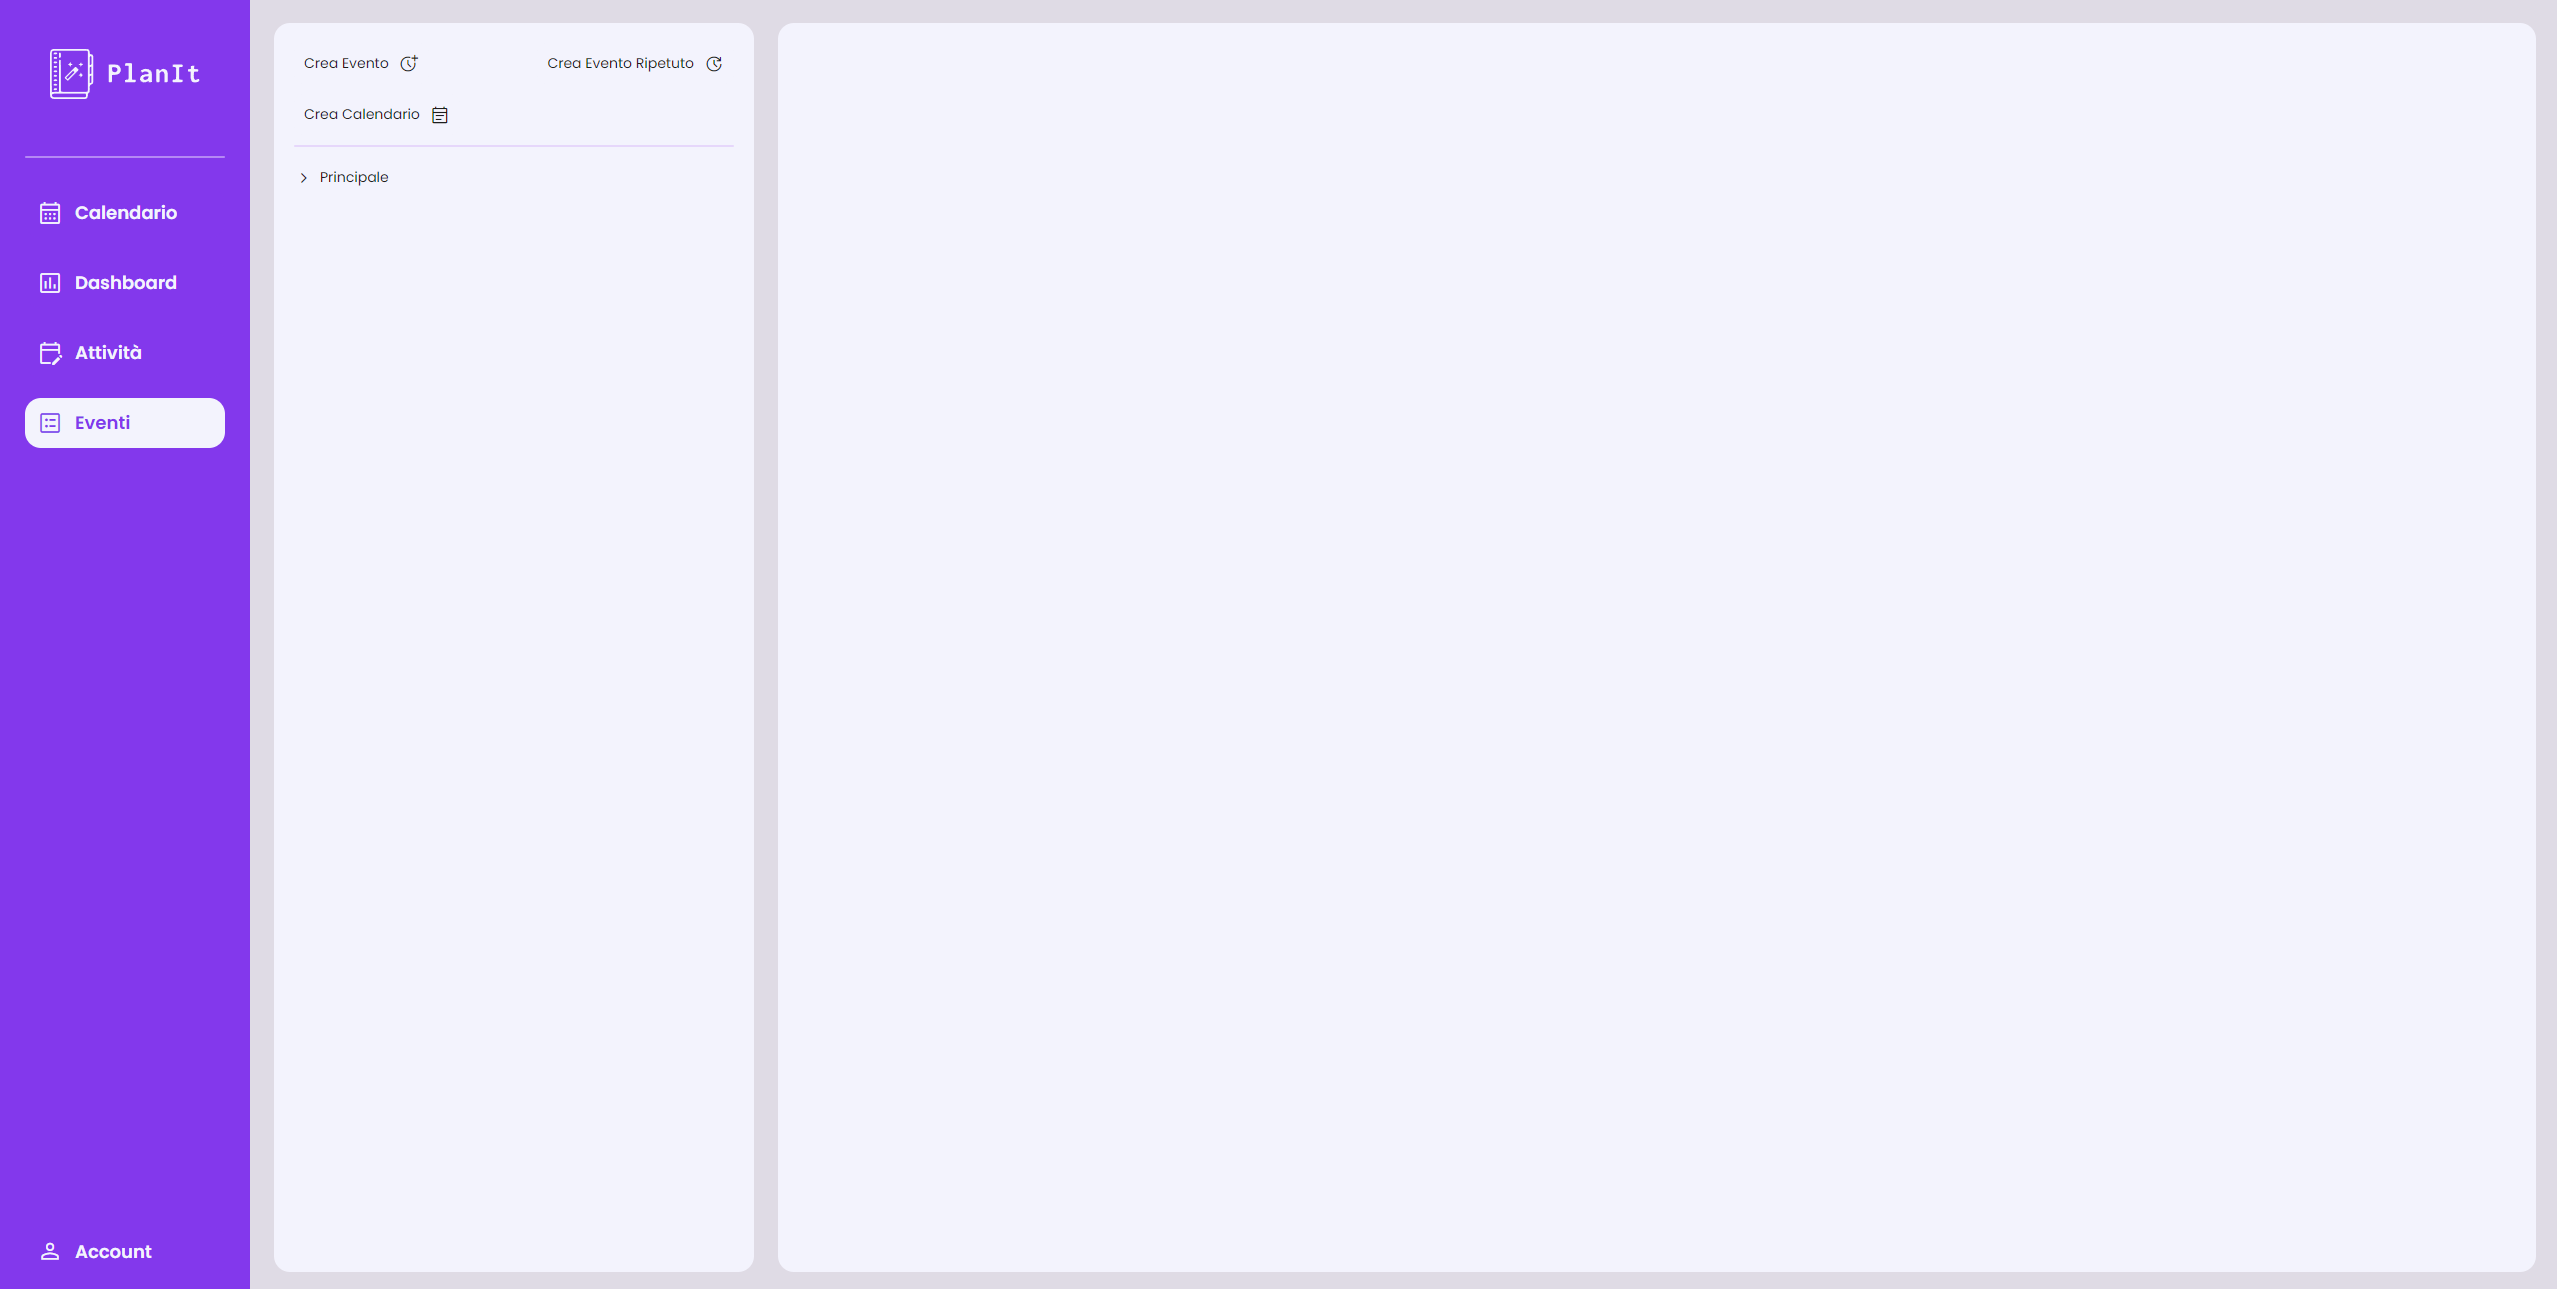
\includegraphics[width=1\textwidth, height=0.3\textheight]{img/png/FrontEnd/Eventi/schermataEventi.png}
    \captionof{figure}{FrontEnd - schermata Eventi}
    \blfootnote{Immagine \href{https://github.com/Life-planner/Documentazione/blob/main/D4/img/png/FrontEnd/Eventi/schermataEventi.png}{PNG} FrontEnd - schermata Eventi}
\end{center}

Nel caso in cui l'utente volesse creare nuovi calendari e nuovi eventi singoli, premendo i tasti in alto a sinistra "Crea Calendario" e "Crea Evento", può visualizzare nella parte destra della schermata i rispettivi form di creazione, identici a quelli che si possono ottenere nella pagina "Calendario".

\begin{center}
    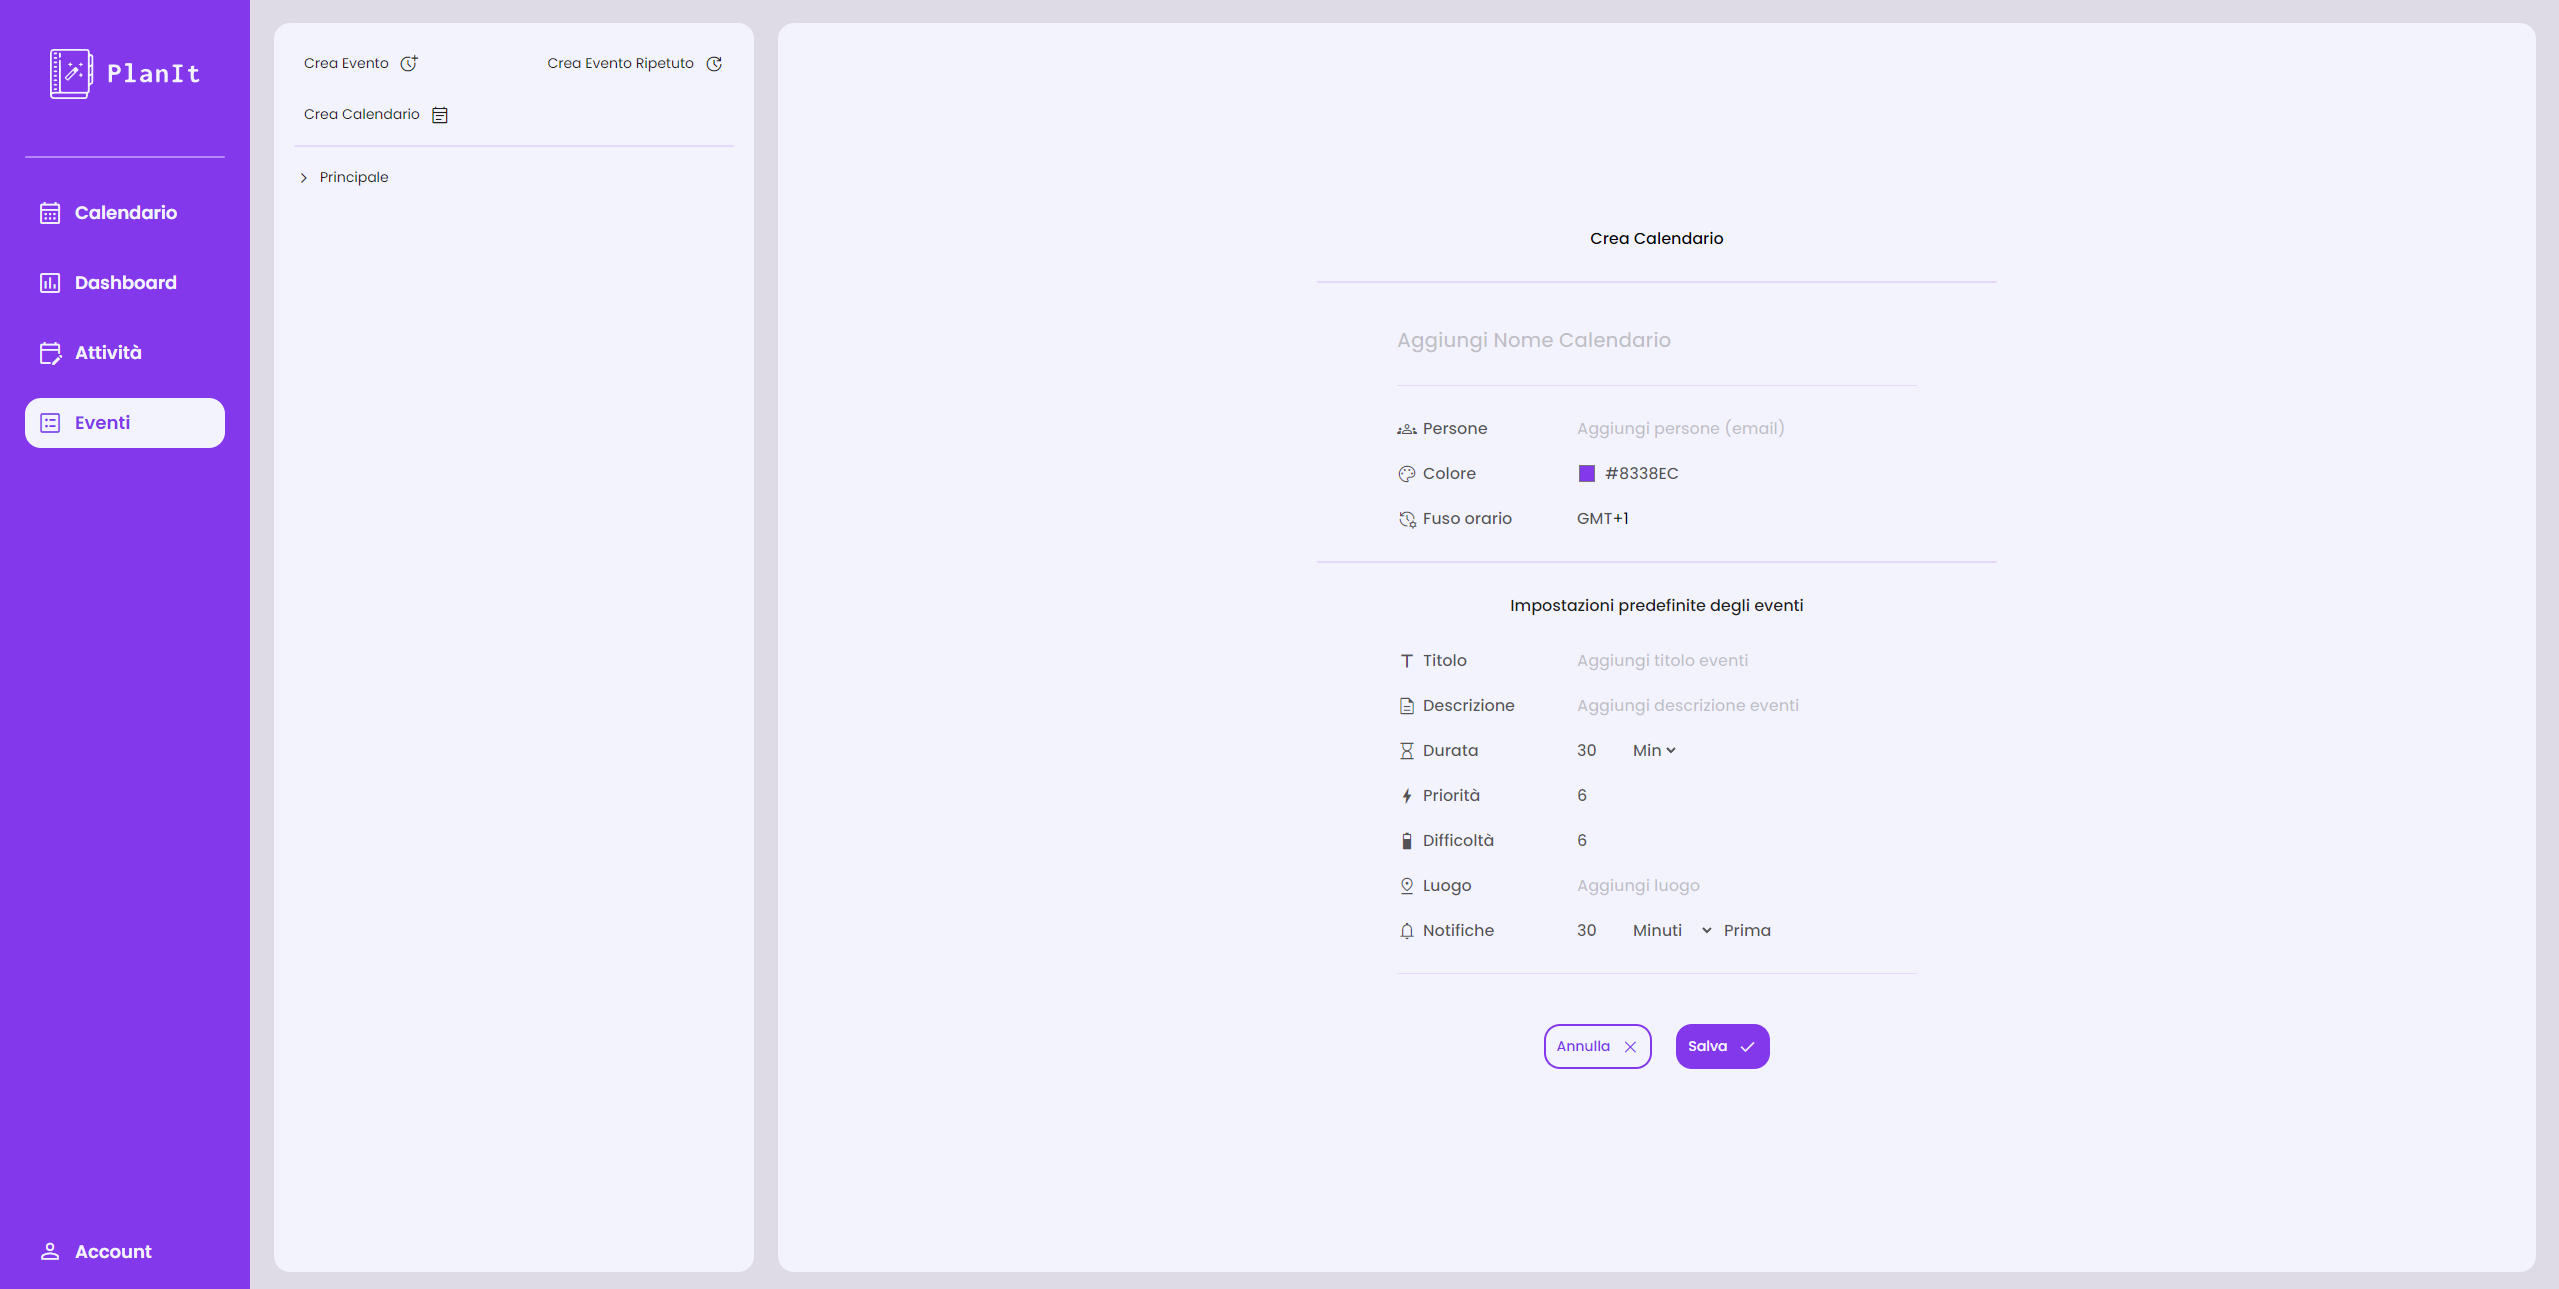
\includegraphics[width=1\textwidth, height=0.3\textheight]{img/png/FrontEnd/Eventi/EventiCreaCalendario.png}
    \captionof{figure}{FrontEnd - "Crea Calendario" da schermata "Eventi"}
    \blfootnote{Immagine \href{https://github.com/Life-planner/Documentazione/blob/main/D4/img/png/FrontEnd/Eventi/EventiCreaCalendario.png}{PNG} FrontEnd - "Crea Calendario" da schermata "Eventi"}
\end{center}

\begin{center}
    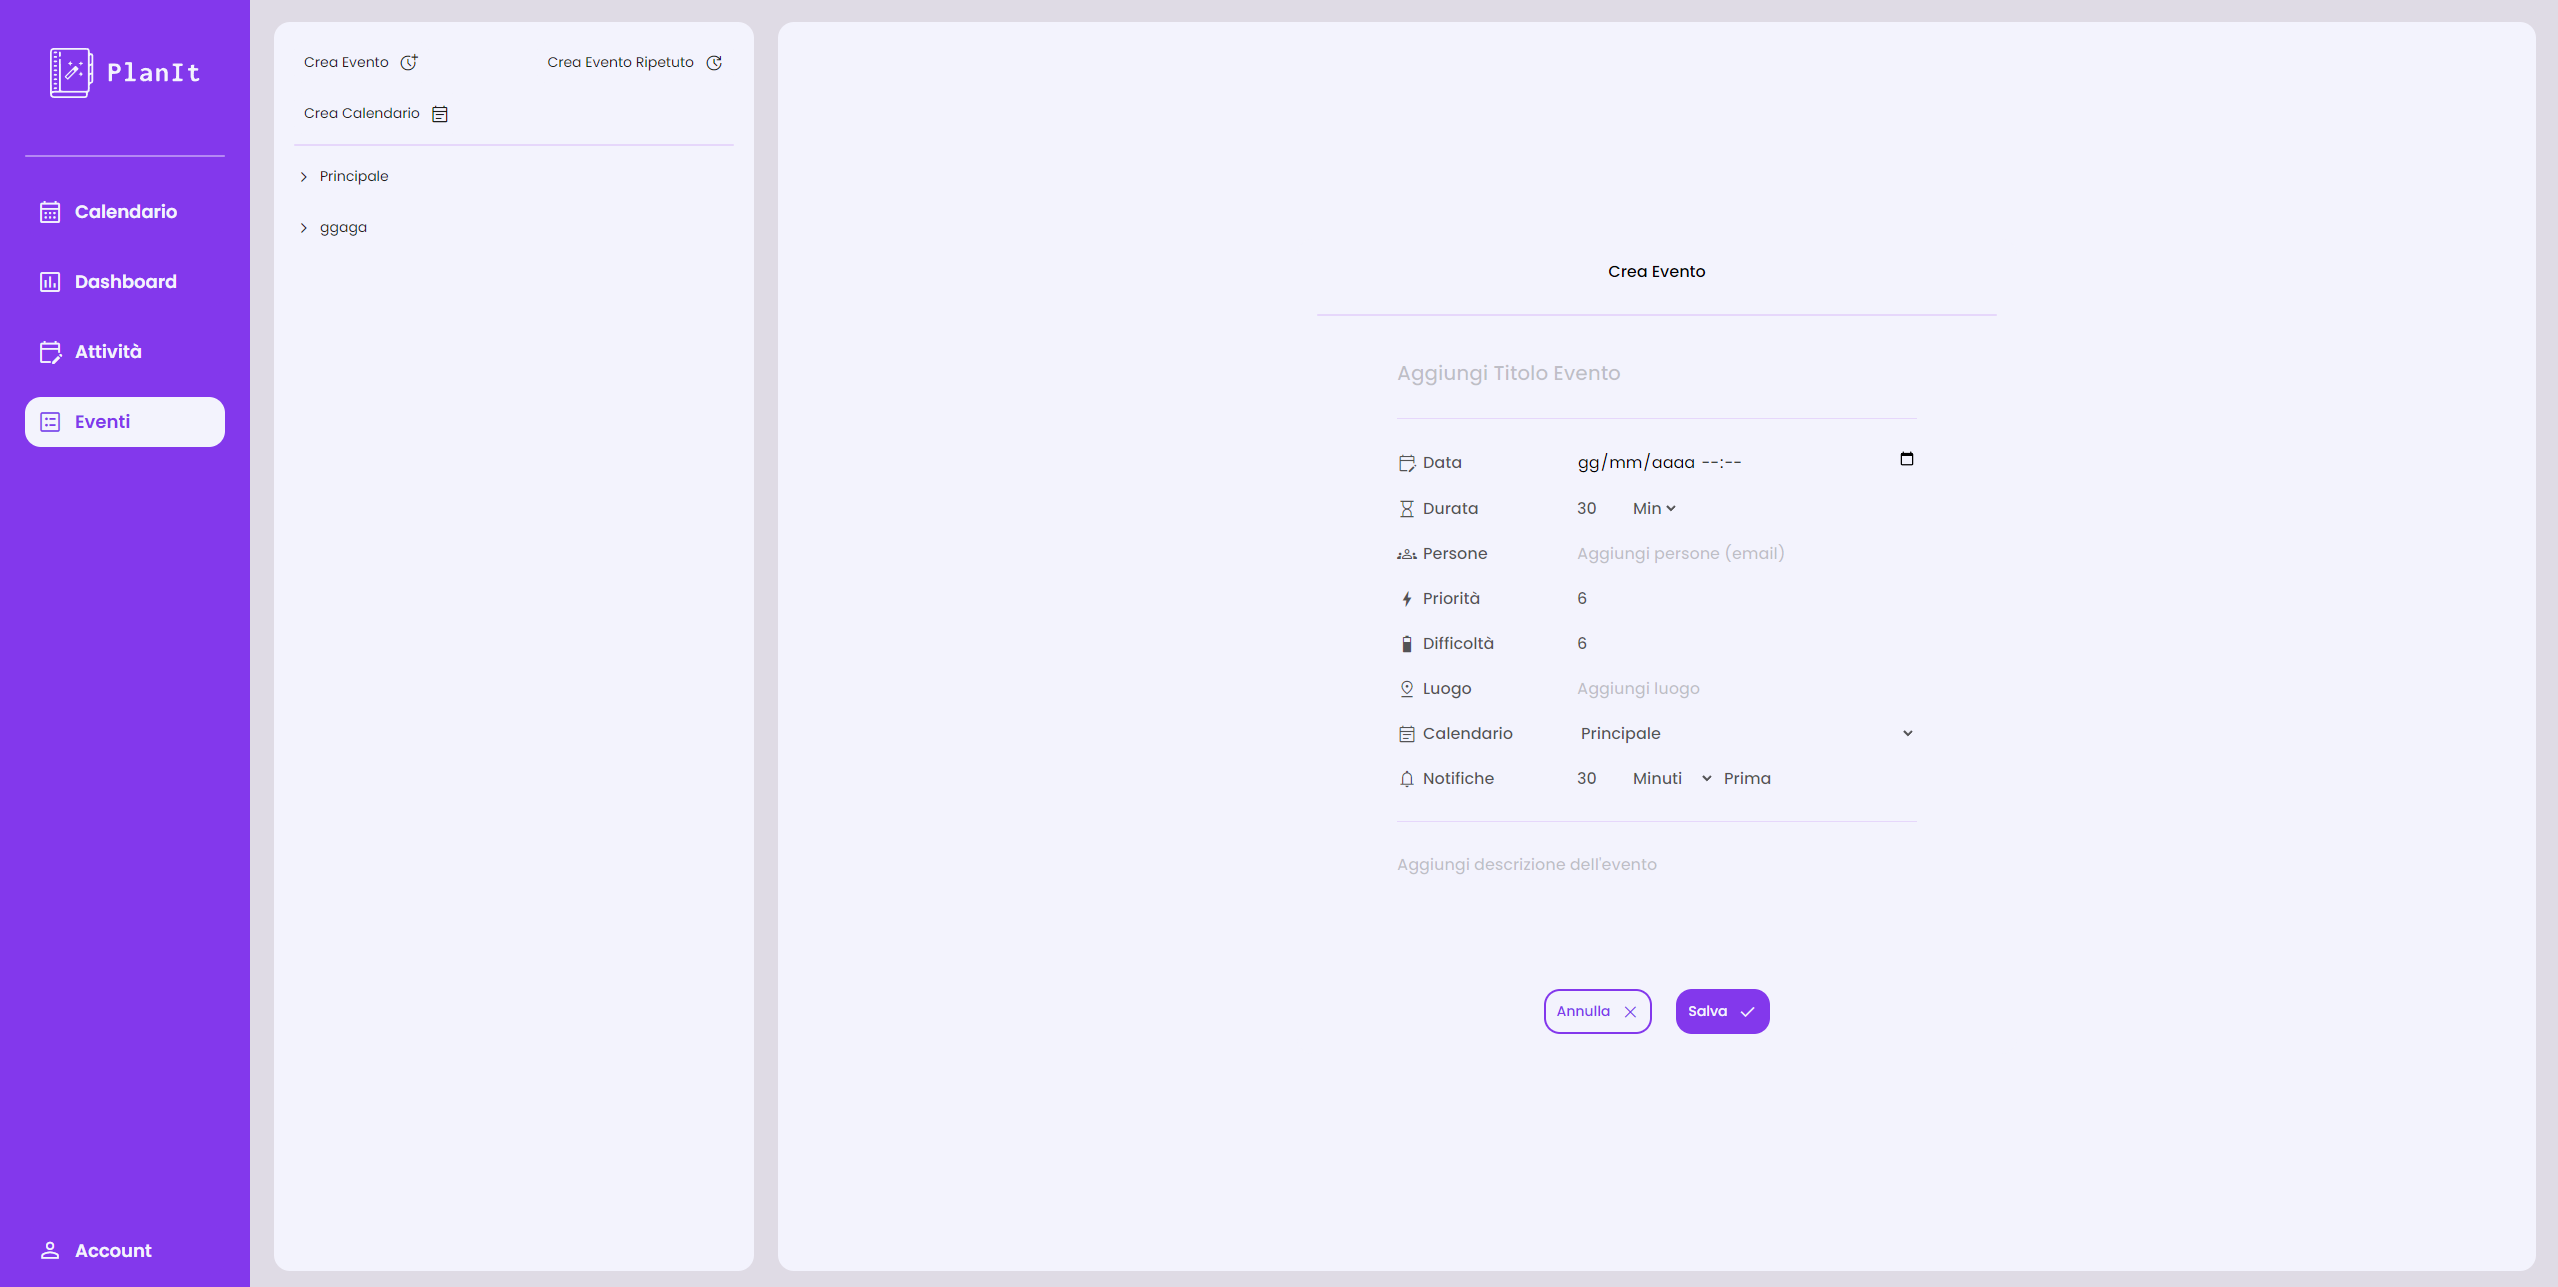
\includegraphics[width=1\textwidth, height=0.3\textheight]{img/png/FrontEnd/Eventi/EventiCreaEvento.png}
    \captionof{figure}{FrontEnd - "Crea Evento" da schermata "Eventi"}
    \blfootnote{Immagine \href{https://github.com/Life-planner/Documentazione/blob/main/D4/img/png/FrontEnd/Eventi/EventiCreaEvento.png}{PNG} FrontEnd - "Crea Evento" da schermata "Eventi"}
\end{center}

\begin{comment}
Dopo, quando l'utente vuole creare un evento ripetuto, ovvero un evento che definiamo presente su più giorni, già in fase di creazione dell'evento, basta che usi il bottone "Crea Evento Ripetuto" per far apparire il form di creazione "Crea Evento Ripetuto". In questo form, tutti i campi sono compilabili, eccetto per "Luogo". Ricordiamo che i campi "nome" e, almeno, una data su cui cade tale evento devono essere sempre presenti, per far andare a buon fine la creazione dell'evento ripetuto. L'utente, mediante le "Impostazioni avanzate", può andare a specificare maggiormente quando cadono tali eventi e in quali orari. Con l'attributo "Durata", l'utente indica per quale periodo di tempo questo evento ripetuto vale e quindi deve essere presente nel calendario.
\end{comment}

L'utente, inoltre, in questa schermata "Eventi" visualizza la lista di calendari. Avendo la possibilità di esplorarli, ovvero visualizzare quali eventi ne fanno parte, può selezionare uno dei suoi eventi per aprire il form di "Modifica Evento". Questo form è uguale a quello di "Crea Evento", ovvero ha gli stessi campi, eccetto che l'utente ha la possibilità di eliminare tale evento selezionato mediante il bottone "Elimina".

\begin{center}
    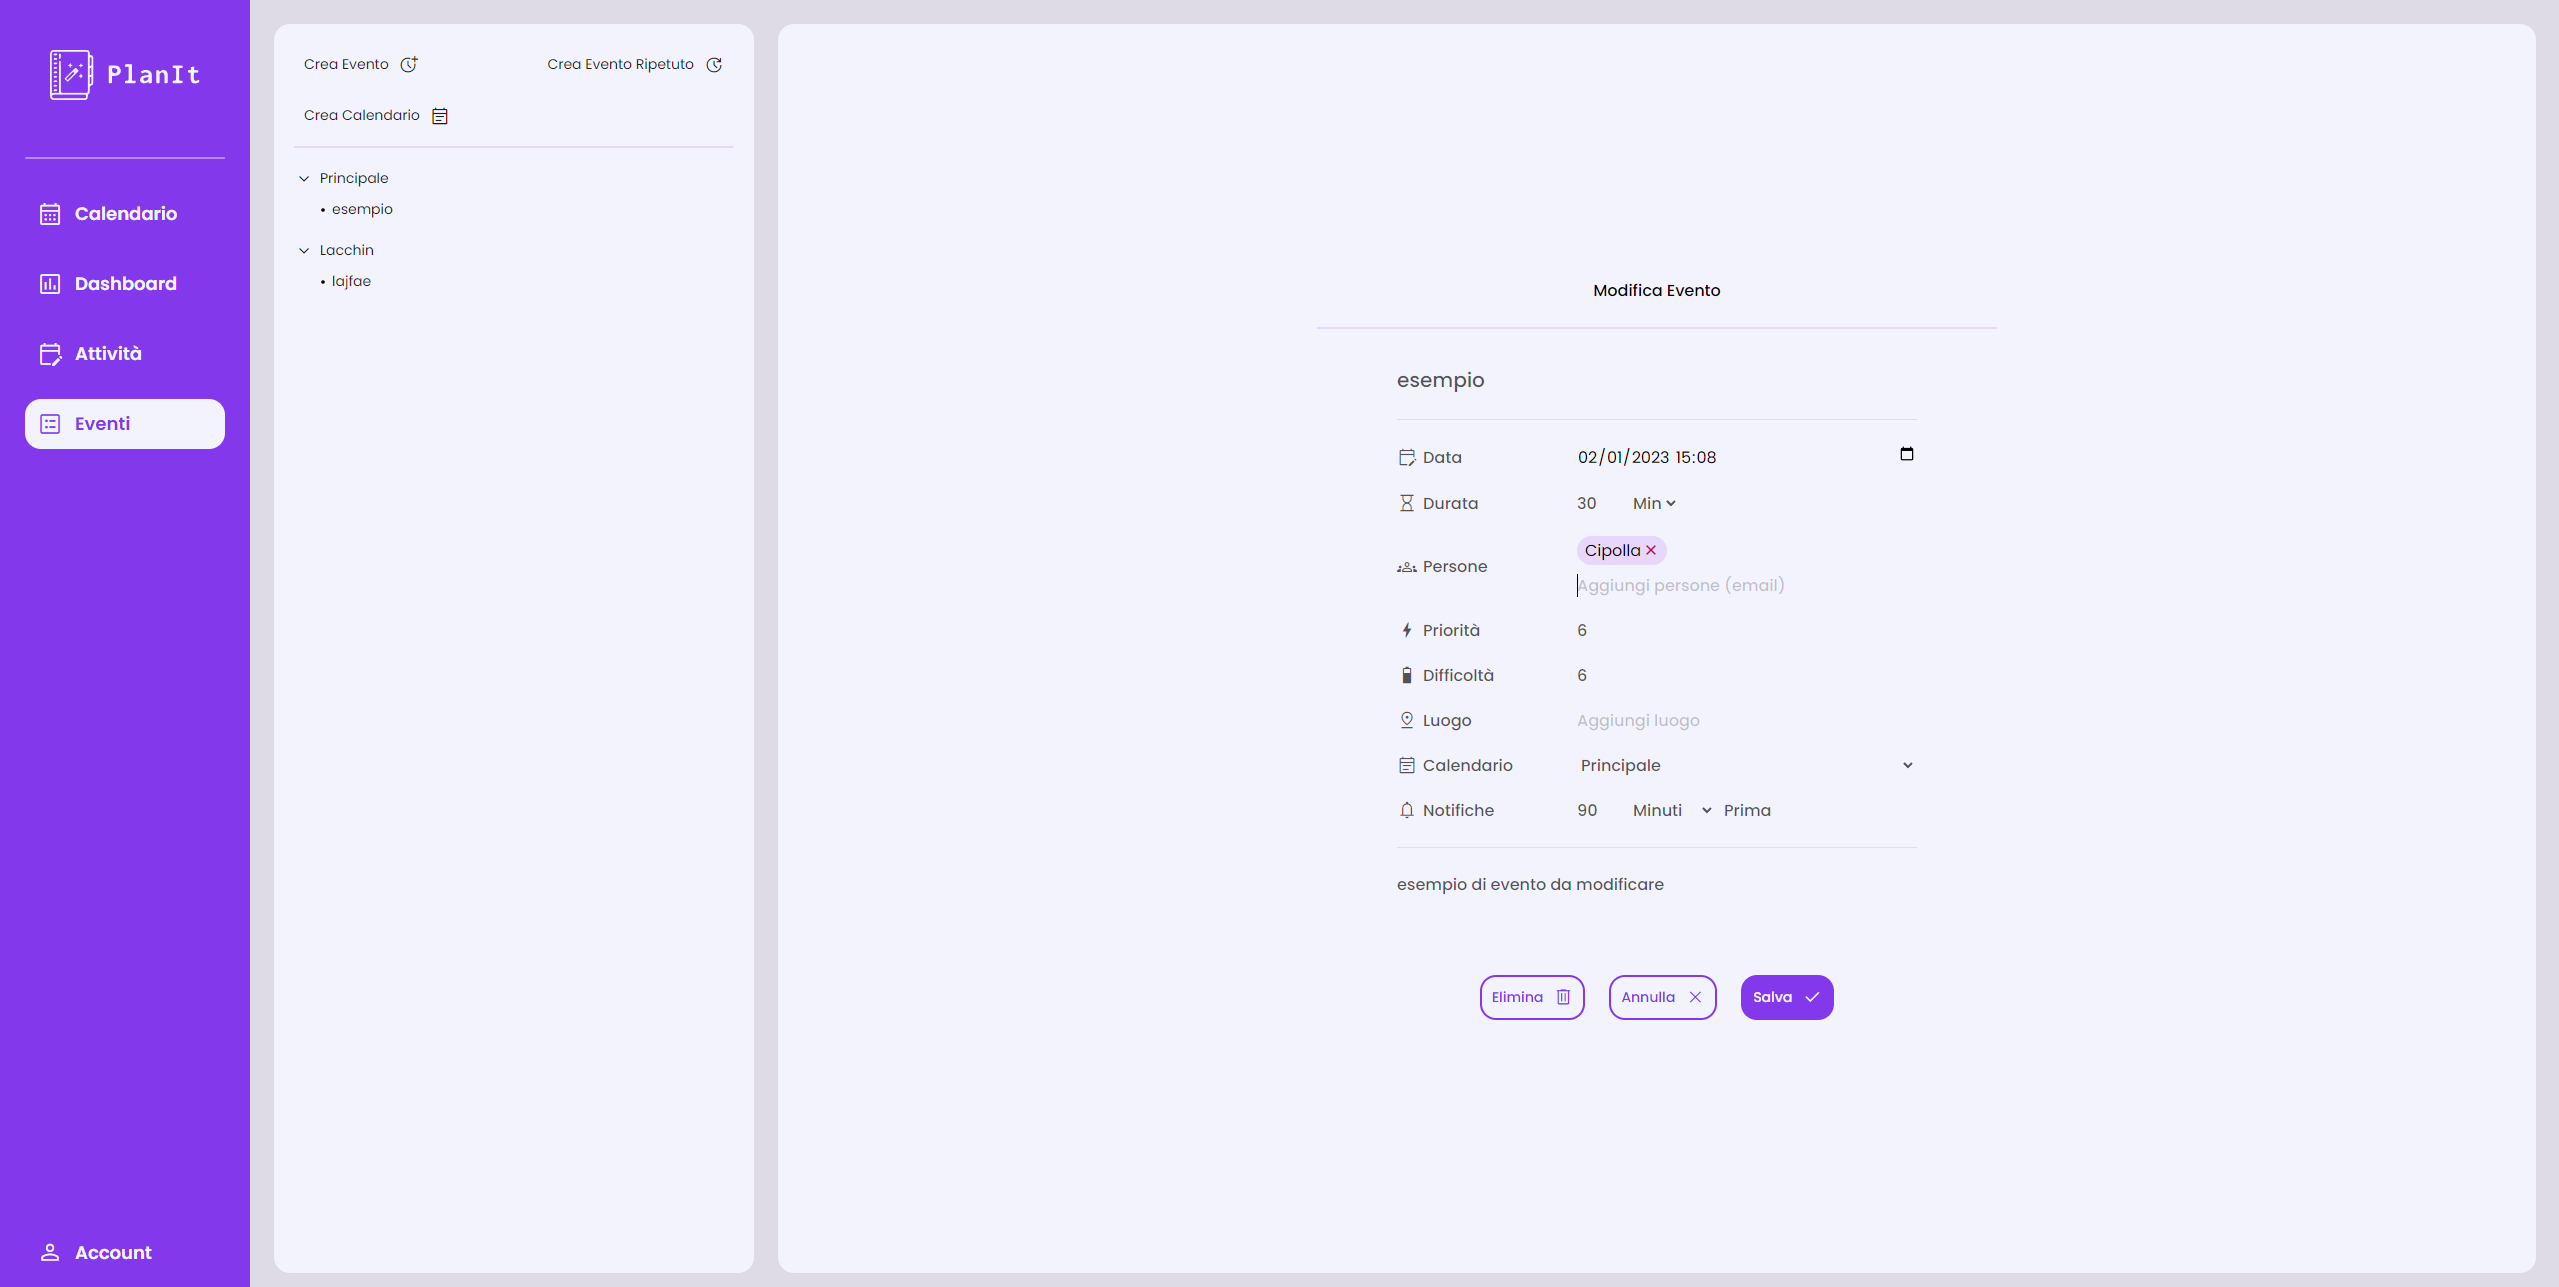
\includegraphics[width=1\textwidth, height=0.3\textheight]{img/png/FrontEnd/Eventi/EventiModificaEvento.png}
    \captionof{figure}{FrontEnd - "Modifica Evento" da schermata "Eventi"}
    \blfootnote{Immagine \href{https://github.com/Life-planner/Documentazione/blob/main/D4/img/png/FrontEnd/Eventi/EventiModificaEvento.png}{PNG} FrontEnd - "Modifica Evento" da schermata "Eventi"}
\end{center}


Infine, selezionando uno dei calendari della lista, si apre il form di "Modifica Calendario", che è identico a quello di "Crea Evento", eccetto per la presenza del bottone "Elimina", che l'utente può utilizzare per eliminare tale calendario.

\begin{center}
    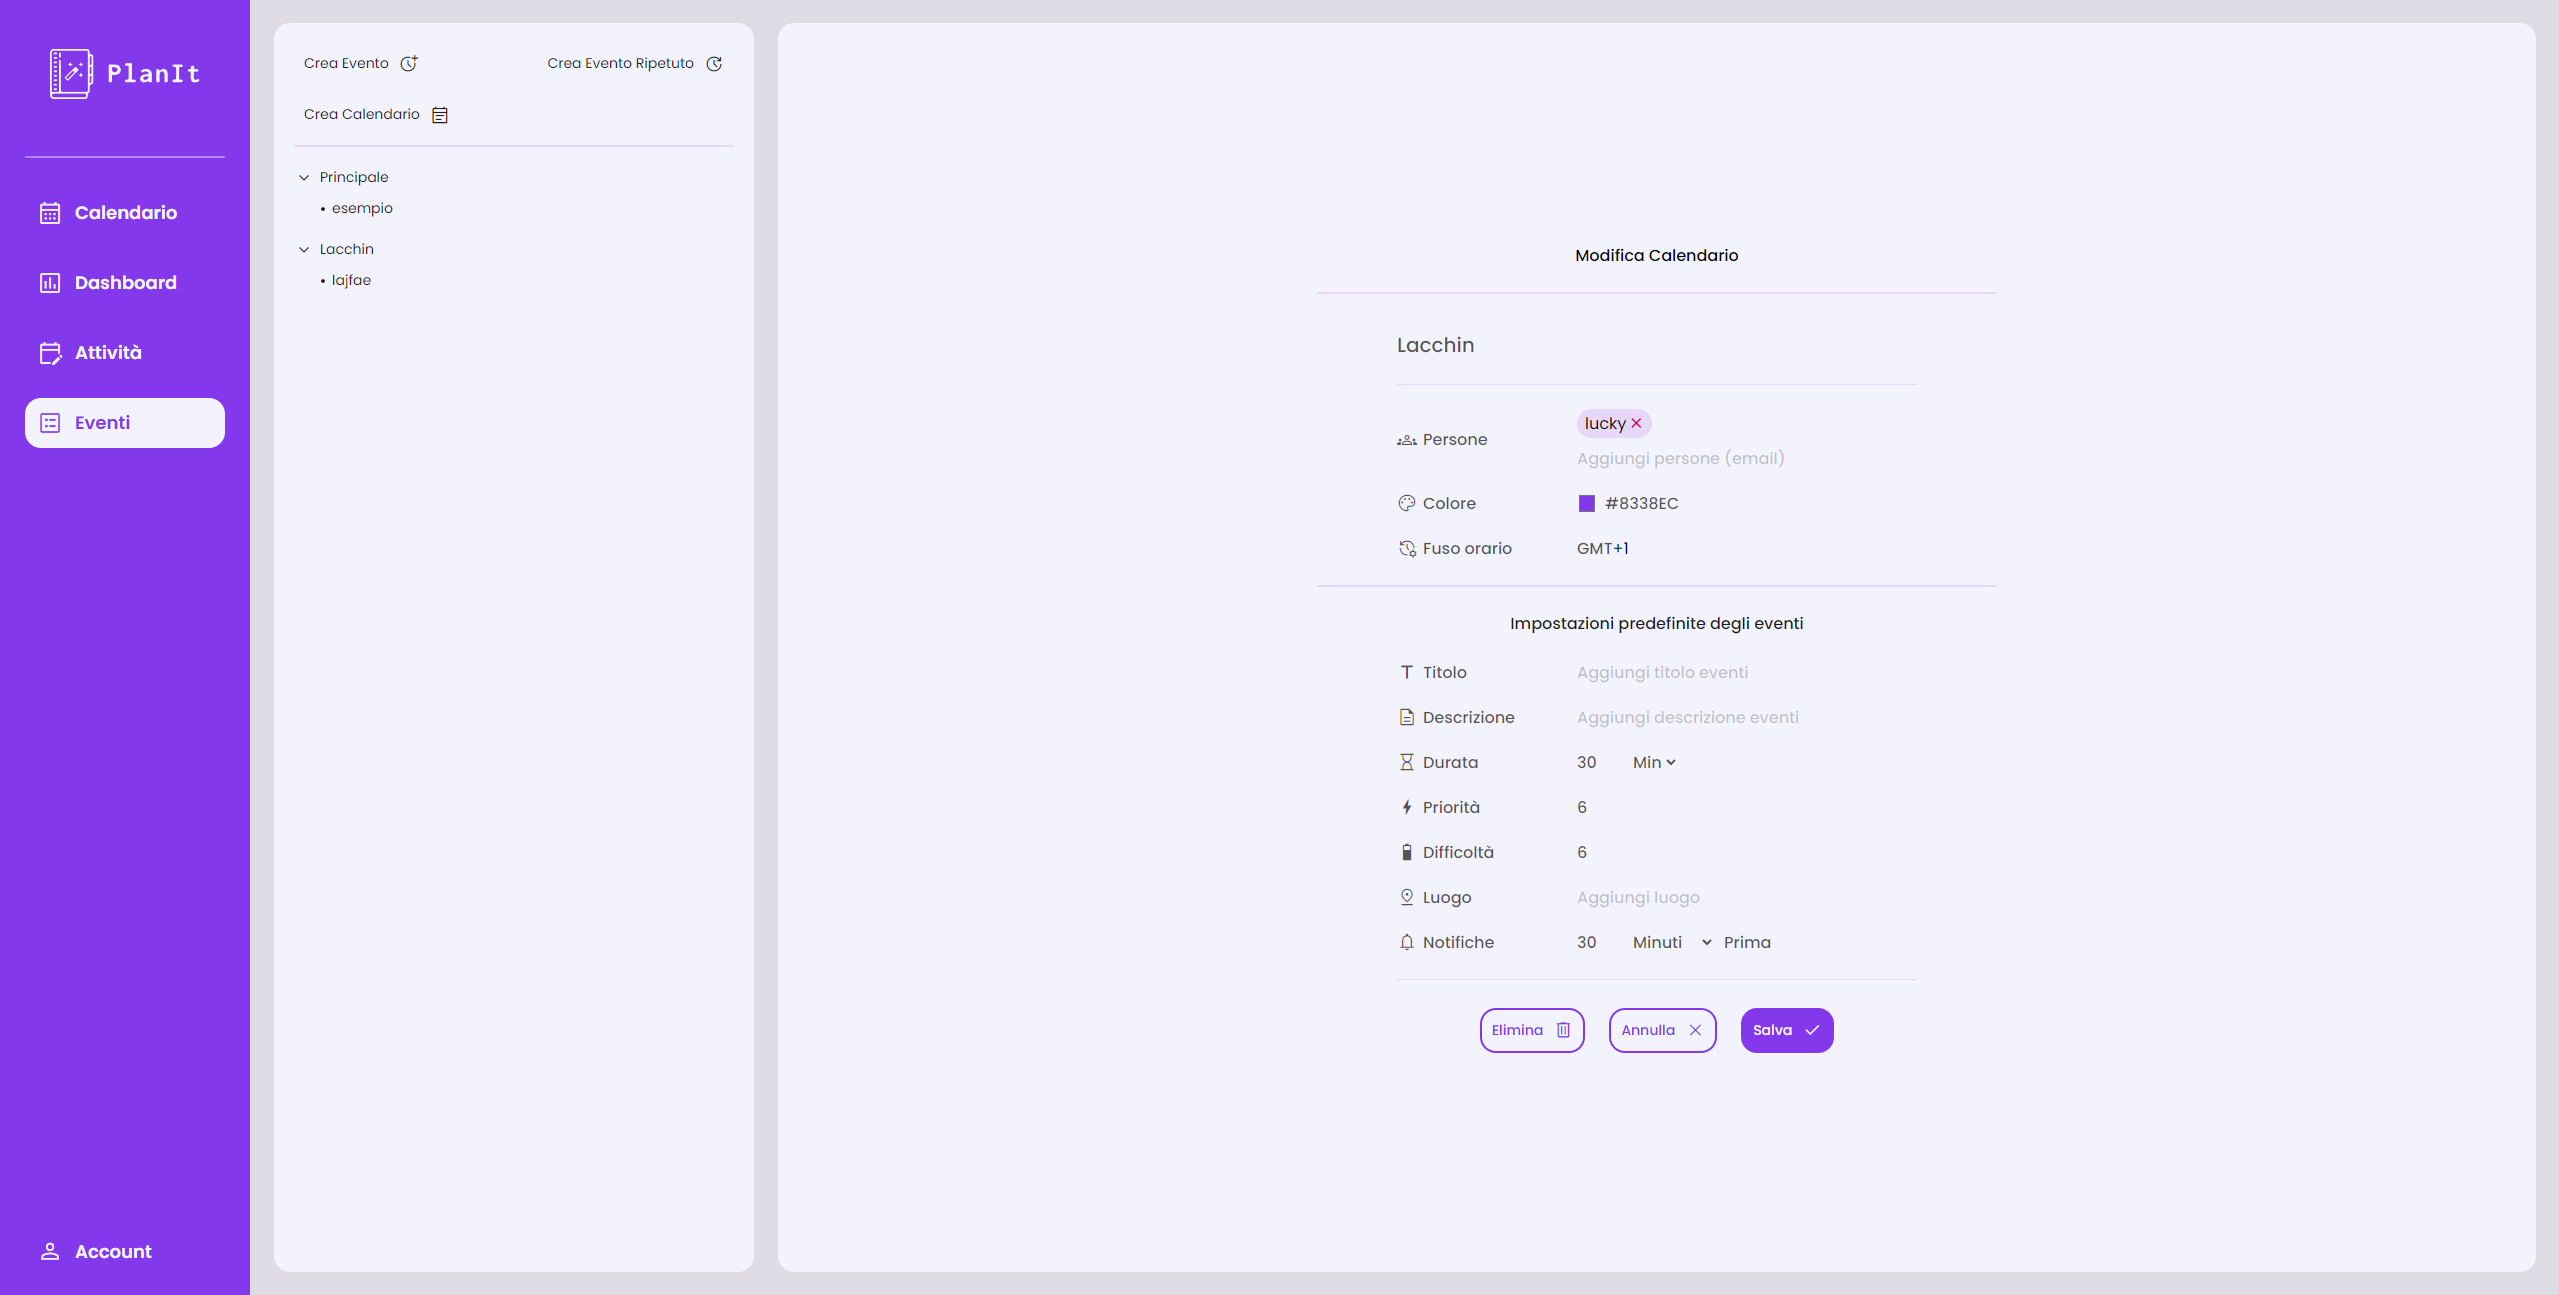
\includegraphics[width=1\textwidth, height=0.3\textheight]{img/png/FrontEnd/Eventi/EventiModificaCalendario.png}
    \captionof{figure}{FrontEnd - "Modifica Calendario" da schermata "Eventi"}
    \blfootnote{Immagine \href{https://github.com/Life-planner/Documentazione/blob/main/D4/img/png/FrontEnd/Eventi/EventiModificaCalendario.png}{PNG} FrontEnd - "Modifica Calendario" da schermata "Eventi"}
\end{center}